% Master's thesis. Generated from THESIS/markdown.
% Layout follows THESIS/thesis-template.
\documentclass[12pt]{book}

\usepackage[a4paper,top=3cm,bottom=3cm,left=3.25cm,right=3.25cm]{geometry}
\usepackage[T1]{fontenc}
\usepackage[utf8]{inputenc}
\usepackage{libertine}
\usepackage[english]{babel}

\usepackage{amsfonts,amssymb,amsmath}
\usepackage{graphicx}
\usepackage{float}
\usepackage{booktabs}
\usepackage{array}
\usepackage{longtable}
\usepackage{csquotes}
\usepackage[style=authoryear,backend=biber,maxcitenames=2,mincitenames=1,giveninits=true,uniquename=false,uniquelist=false,dashed=false]{biblatex}
\addbibresource{bib/bibliography.bib}
\DeclareDelimFormat{finalnamedelim}{\addspace\&\space}

\usepackage{hyperref}
\hypersetup{
  hidelinks,
  pdftitle={Unsupervised State Bucketing for Mixture of Experts in Resource-Constrained Chess Engines},
  pdfauthor={Omar Cusma Fait}
}
\usepackage{xurl}
\usepackage{emptypage}
\usepackage{fancyhdr}
\usepackage{tocbibind}
\usepackage{listings}
\usepackage{caption}
\usepackage{subcaption}
\usepackage{lmodern}
\usepackage{microtype}

\lstset{
  basicstyle=\ttfamily\small,
  breaklines=true,
  columns=fullflexible,
  frame=single,
  language=Python,
  showstringspaces=false
}

\lhead{}
\fancyhead[R]{\empty}
\renewcommand{\headrulewidth}{0pt}
% Number floats by chapter so ``Table 5.1'' in the text matches the caption.
\renewcommand{\thefigure}{\thechapter.\arabic{figure}}
\renewcommand{\thetable}{\thechapter.\arabic{table}}
\setcounter{secnumdepth}{3}
\setcounter{tocdepth}{2}
\setlength{\headheight}{15pt}
\setlength{\parindent}{0pt}
\setlength{\parskip}{0.65em plus 0.15em minus 0.1em}
\setlength{\emergencystretch}{2em}
\let\cleardoublepage\clearpage

\begin{document}
\hypersetup{pageanchor=false}
\thispagestyle{empty}
\begin{center}

\includegraphics[width=.42\textwidth]{../thesis-template/logo_centenario-eps-converted-to.pdf}\\[1.2cm]
{\LARGE\textsc{Universit\`a degli Studi di Trieste}}\\
\rule{\textwidth}{0.1mm}\\[0.4em]
{\large\textsc{Dipartimento di Scienze Economiche, Aziendali, Matematiche e Statistiche -- DEAMS}}\\[1.6em]
Corso di Laurea Magistrale in Data Science and Artificial Intelligence\\
Curriculum: Foundations of AI and ML\\[2.2em]
{\textsc{Tesi di laurea magistrale}}\\[2.2em]
{\LARGE\textbf{Unsupervised State Bucketing for Mixture of Experts in Resource-Constrained Chess Engines}}\\
\end{center}
\vspace{1.6cm}
\begin{tabular}[t]{l}
Laureando:\\
\textbf{Omar Cusma Fait}\\
\textsc{Matricola: SM3800018}
\end{tabular}
\hfill
\begin{tabular}[t]{l}
Relatore:\\
\textbf{Prof.\ Alessio Ansuini}\\[1em]
Correlatore:\\
\textbf{Prof.\ Marco Zennaro}\\
\textsc{ICTP}
\end{tabular}
\vfill
\begin{center}
\rule{8cm}{0.1mm}\\[0.8em]
ANNO ACCADEMICO 2025--2026
\end{center}
\clearpage

\thispagestyle{empty}
\vspace*{0.42\textheight}
\begin{center}
\textit{Divide and conquer.}
\end{center}
\clearpage

\hypersetup{pageanchor=true}
\frontmatter
\pagestyle{plain}
\chapter{Abstract}
In the context of board games, a common approach for improving model performance is to partition the state space and allocate distinct experts to each region. While this is the central idea behind \emph{Mixture of Experts} (MoE) architectures, the bucketing is often defined manually, requiring domain-specific expertise, and yielding potentially suboptimal partitions.

We investigate and compare several approaches to extending the \emph{Efficiently Updatable Neural Networks} (NNUE) paradigm beyond its conventional formulation, with a particular focus on techniques that have been successfully explored in other areas of machine learning but remain relatively uncommon in NNUE-based chess engines. Mixture-of-Experts architectures are a natural extension for chess evaluation that allows multiple specialized heads to share a common NNUE representation. We also explore sample-gradient-based partitioning, using the gradients of individual training samples to identify groups of positions with similar learning requirements, an approach more commonly studied in large-scale language models and other deep learning settings. Finally, in an effort to make the NNUE architecture more applicable to other fields, we experiment with making its conventional accumulator a learned world model of the game.

The results highlight different trade-offs between the investigated approaches. L1-based clustering combined with a Mixture-of-Experts architecture significantly improves evaluation performance, while introducing only a minor increase in memory usage and inference cost; the lightweight dispatcher accurately reproduces the learned partition. In contrast, sample-gradient-based partitioning is difficult to exploit at inference time, since the gradients depend on the unknown true value of the position, and a lightweight dispatcher struggles to approximate the resulting complex partition. Finally, the world-model approach shows that an NNUE-like architecture can be trained without feedback from a teacher engine or game outcomes, although the unsupervised training objective can reduce evaluation strength. At the same time, learning the world model makes the training process more efficient by shifting a substantial part of the learning effort to the shared representation.


\tableofcontents
\listoffigures
\listoftables

\mainmatter
\pagestyle{fancy}
% !TeX root = ../main.tex
\chapter{Introduction}

\section{Motivation}

% Motivation - tight resources
A chess engine evaluates a large number of positions during search, and the quality of this evaluation directly affects the strength of the resulting moves. On a desktop system, this evaluation can rely on relatively large neural networks. On a microcontroller, memory, computation, and latency constraints impose tighter limits on the size and cost of the evaluation function. The evaluation function must be small and cheap to run at every node of an alpha-beta search. \emph{Efficiently Updatable Neural Networks} (\textbf{NNUE}) architectures have become a widely used approach for neural evaluation in modern chess engines \parencite{nasu2018}.

\begin{figure}[H]
	\centering
	\includegraphics[width=0.86\textwidth]{../thesis-plots/nnue_incremental_update.png}
	\caption{Incremental update of the NNUE accumulator.}
	\label{fig:nnue-incremental-update-1}
\end{figure}

% bucketing and MoE
A single shallow head must represent positions arising from substantially different tactical and positional regimes. This raises the question of whether different regions of the state space could benefit from specialized heads. Different positions may require understanding of very diverse aspects of the game. Mixture-of-Experts (\textbf{MoE}) evaluation provides a natural framework for this form of specialization \parencite{shazeer2017}: partition the state space into buckets, and assign an \emph{expert head} to each region, while keeping a shared representation. Common chess-engine bucketing strategies rely on manually designed features such as piece count, king location, or game phase \parencite{nasu2018}. Those rules are cheap and interpretable, but they are game-specific heuristics and are not necessarily optimal. They encode what a programmer thinks is a distinct regime, not what the model actually needs in order to specialise.

% Unsupervised alternatives & Literature gap
Unsupervised alternatives exist. Clustering hidden-layer activations groups positions that look similar in the eyes of the network; however, representation similarity does not necessarily reflect similarity in the learning signal. Recent developments in large language models---such as \textbf{ELREA} \parencite{li2025} and \textbf{GradientSpace} \parencite{sridharan2025}---demonstrate that grouping samples by their gradient directions can effectively guide expert specialization. Nevertheless, these techniques target massive LLMs and do not translate directly to embedded environments, where routing overhead and memory footprints are severely restricted. 

This motivates defining partitions via parameter-space directions induced by individual training samples, adapting sample-gradient clustering into a lightweight, data-driven framework suitable for on-device NNUE evaluation without relying on chess-specific heuristics.

\begin{figure}[H]
	\centering
	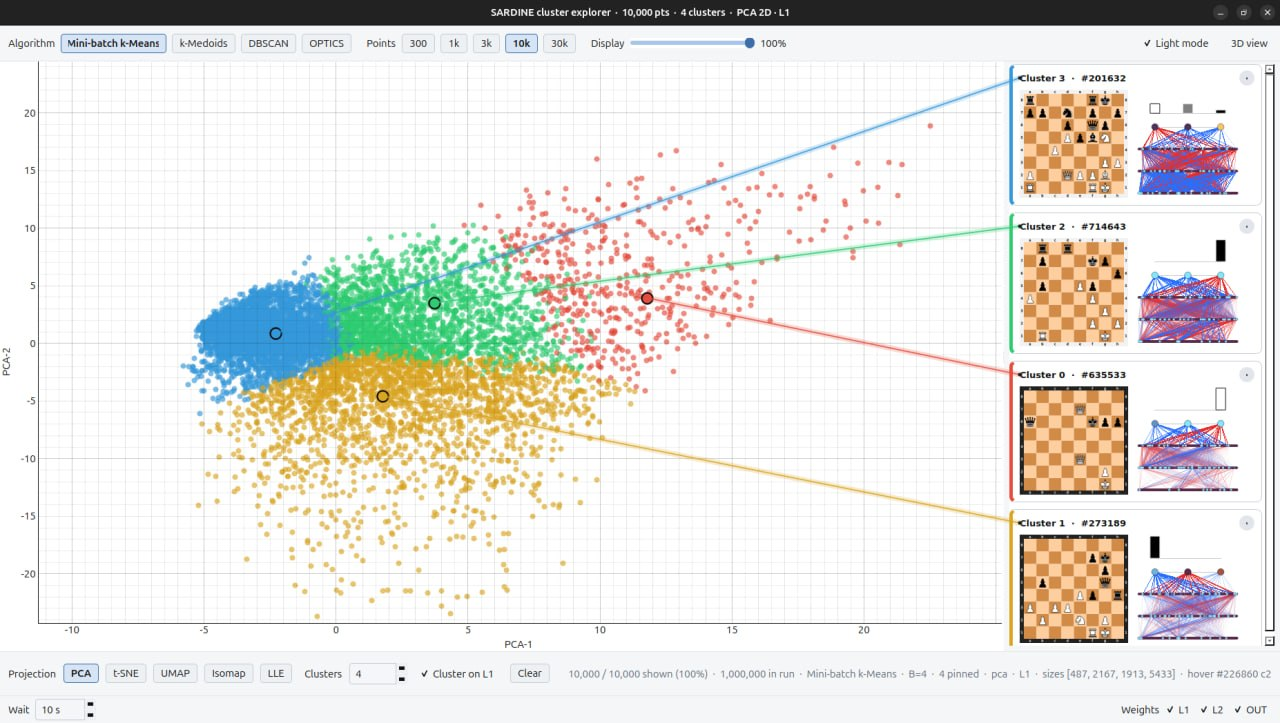
\includegraphics[width=0.86\textwidth]{../thesis-plots/L1_clustering.jpg}
	\caption{Positions clustered by L1 activations and projected to two dimensions.}
	\label{fig:l1-clustering-2}
\end{figure}

\section{Scope of the Thesis}

The central problem addressed in this thesis is the investigation of data-driven approaches for improving neural chess evaluation under the tight memory and computational constraints of embedded devices. In particular, this work explores how the NNUE architecture can be extended to represent different forms of specialization, while retaining the extreme latency efficiency demanded by deep alpha-beta search.

This research investigates how advanced machine learning techniques can be synthesized to enhance neural evaluation. Specifically, we evaluate replacing the standard NNUE accumulator with a learned world-model encoder, compare handcrafted bucketing against unsupervised clustering based on L1 activations and sample gradients, and contrast end-to-end Mixture-of-Experts routing with the Hard MoE paradigm.

These approaches are evaluated from both a learning and deployment perspective. The overarching research question is whether ideas from diverse machine learning paradigms can offer favorable trade-offs between specialization, evaluation quality, and execution efficiency on resource-constrained hardware.

\section{Contributions}

The main contributions of this thesis are summarized as follows:

\begin{itemize}
	\item \textbf{Data-driven State-space Partitioning:} We adapt sample-gradient clustering to NNUE evaluation, creating an unsupervised state-space bucketing scheme that avoids reliance on domain-specific heuristics.
	\item \textbf{Lightweight Routing Mechanism:} We introduce a two-phase architecture where computationally expensive gradient clustering is restricted to offline training, while a lightweight dispatcher predicts expert assignment from frozen accumulator activations during inference.
	\item \textbf{World-Model Integration:} We demonstrate the feasibility of replacing traditional hand-crafted accumulators with a learned world-model encoder, assessing its impact on representation learning and training efficiency.
	%% \item \textbf{Embedded Benchmarking and Deployment:} We quantize and integrate the proposed models into the \emph{Cfish} engine, providing an empirical trade-off analysis between evaluation strength, memory footprint, and search speed on microcontroller hardware.
	\item \textbf{Embedded Benchmarking and Deployment:} We design a quantized integration path for the proposed models in the Cfish engine, specifying the memory layout, integer arithmetic, and inference procedure required for deployment on microcontroller hardware. The empirical analysis of evaluation strength, memory footprint, and search speed is left to future work.
\end{itemize}

\section{Thesis Outline}

The remainder of this thesis is organized as follows:

\begin{itemize}
	\item \textbf{Chapter 2 (Background and Related Work):} Reviews the fundamentals of chess evaluation functions, NNUE architectures, Mixture-of-Experts, and existing sample-gradient specialization techniques.
	\item \textbf{Chapter 3 (Methodology and Experimental Pipeline):} Details the proposed unsupervised bucketing algorithms, sample-gradient clustering, the world-model encoder architecture, and the lightweight routing mechanism.
	\item \textbf{Chapter 4 (Implementation):} Describes the dataset generation, network training, model quantization, and integration with the Cfish engine on embedded hardware.
	\item \textbf{Chapter 5 (Experimental Results):} Presents empirical evaluations regarding expert specialization, evaluation quality, and latency trade-offs compared to single-head and heuristic baselines.
	\item \textbf{Chapter 6 (Discussion):} Interprets the empirical findings, analyzes the routing bottlenecks, and discusses the limitations and generalization of the proposed methods.
	\item \textbf{Chapter 7 (Conclusion and Future Work):} Summarizes the primary findings, discusses current limitations, and outlines directions for future research.
\end{itemize}

% !TeX root = ../main.tex
\chapter{Background and Related Work}

\section{Foundations of Neural Chess Evaluation}

\subsection{The Role of Evaluation and Classical Approaches}
At the core of every chess engine lies an evaluation function $f: \mathcal{S} \rightarrow \mathbb{R}$ that assigns a scalar value to a board position $s \in \mathcal{S}$, indicating the expected outcome from that position (typically from the perspective of the player to move). This value guides the search algorithm -- usually a variant of \textbf{alpha-beta search} with iterative deepening -- by pruning unpromising branches and selecting the most best moves.

For decades, chess evaluation functions were handcrafted. A classical evaluator is a weighted linear combination of chess-specific features:
\[
f(s) = \sum_{k} w_k \cdot \phi_k(s)
\]
where $\phi_k(s)$ are feature functions and $w_k$ are scalar weights. Typical features include material balance, piece-square tables (PSTs), mobility, king safety, and pawn structure. Chess experts carefully tuned these features over decades, using a combination of intuition, empirical testing, and later automated optimization techniques.

Traditional engines typically evaluate a position using a scalar value called \emph{centipawn}. Positive values indicate an advantage for White, while negative values indicate an advantage for Black. The name hints at the fact that the value of a pawn corresponds to 100 centipawns, but this is not entirely accurate, as the value of each piece changes dynamically depending on the position. Therefore, interpretability is a crucial weakness of this metric. Similarly, since centipawns hint at material advantage, they lose meaning when the probability of a color winning is extreme, usually capping at around 5000 centipawns.

% todo reference to some centipawn discussion online?

A notable example of a highly tuned classical evaluator is \textbf{PeSTO} (Piece-Square Tables Only), an evaluation function by Ronald Friederich that relies exclusively on piece-square tables. Its tables are optimized via \emph{Texel}'s tuning method and use a \emph{tapered evaluation} that interpolates between separate opening and endgame tables based on the game stage. Conceptually, PeSTO is equivalent to a linear feed-forward network: both compute a weighted sum of piece-square features, with no interaction terms between pieces. While still a handcrafted linear form, PeSTO demonstrates how far such classical approaches can be pushed through data-driven tuning \parencite{friederichpesto}.

\begin{figure}[H]
	\centering
	\includegraphics[width=0.86\textwidth]{../thesis-plots/pesto_pawn_mg.png}
	\caption{PeSTO middlegame pawn table, in centipawns.}
	\label{fig:pesto-pawn-mg-1}
\end{figure}

While classical evaluators are extremely fast, they suffer from fundamental limitations. Human-designed features encode human assumptions about chess, which may not align with the optimal understanding of the game. Moreover, these models do not take into account the positions as a whole; the same parameters give a positional bonus for a central knight whether the position is a quiet middlegame or a tactical melee, even though the knight's practical value may differ dramatically across phases.

Classical evaluators are also vulnerable to the \emph{horizon effect}. A search algorithm constrained to a fixed depth evaluates positions at the search frontier as if the game were stable at that point. If a tactical sequence begins at the horizon but extends one ply further, the engine cannot see the consequences and may assign an inaccurate evaluation. Classical evaluators, which rely on static features, are particularly susceptible: they treat a position at the horizon as if it were quiet, ignoring the tactical possibilities that would unfold if the search continued.

\subsection{The Shift to Neural Evaluation}
The limitations of handcrafted features led to the adoption of neural networks as evaluation functions. \textbf{AlphaZero} \parencite{silver2018} demonstrated that a deep convolutional network, trained via self-play reinforcement learning, could surpass the best classical engines. However, these networks are computationally expensive -- requiring millions of operations per evaluation -- making them unsuitable for resource-constrained devices or for engines that must evaluate millions of positions per second.

AlphaZero's value head outputs a scalar $v\in[-1,+1]$, interpreted as the expected game outcome from the current player's perspective. This scalar is the training target for the value network. However, AlphaZero's training and inference rely on \textbf{Monte Carlo Tree Search (MCTS)}, which builds a search tree by repeatedly simulating trajectories and using the neural network to evaluate leaf nodes. This process requires many forward passes of the network per position, making it computationally expensive and poorly suited for engines that evaluate millions of positions per second with alpha-beta search. The AlphaZero network itself is a deep residual architecture with millions of parameters, requiring floating-point operations and substantial memory, which far exceeds the capacity of microcontrollers \parencite{browne2012}.

% todo reference to MCTS?

\begin{figure}[H]
	\centering
	\includegraphics[width=1.0\textwidth]{../thesis-plots/mcts_wiki.png}
	\caption{The four steps of Monte Carlo tree search.}
	\label{fig:mcts-wiki-2}
\end{figure}

\subsection{NNUE: A Hybrid Approach}
To bridge the gap between the representational power of neural networks and the speed of classical evaluators, the \textbf{Efficiently Updatable Neural Network (NNUE)} architecture was introduced in the \emph{shogi} engine \emph{YaneuraOu} and later adopted by \emph{Stockfish}. 

% todo one phrase for shogi?

The architecture consists of two ingredients: a sparse first layer called the \emph{accumulator}, and a small fully-connected head. The accumulator layer maps a binary representation of the board to a hidden representation $h \in \mathbb{R}^{d}$ via $h = W_{L1} \cdot x$, where $x$ is a sparse binary vector indicating the presence of pieces on squares. The key insight is that a chess move changes only a few bits of $x$, so $h$ can be updated incrementally by adding and subtracting the corresponding columns of $W_{L1}$, rather than by recomputing the entire matrix-vector product from scratch. This makes the cost of the computation of L1 negligible.

The second ingredient, the fully connected head, is typically one or two hidden layers followed by an output layer, mapping $h$ to the position value. A complete NNUE engine leverages alpha-beta search with iterative deepening: starting from the root position, the engine searches deeper and deeper, using the NNUE evaluation at leaf nodes to guide the pruning and ordering of moves. At every node of this search tree, the evaluation function is called hundreds or thousands of times, making its speed critical. Being trained on enormous amounts of data, a NNUE does not suffer from the horizon problem as much as a PST does.

Beyond the standard NNUE formulation, recent trends in machine learning suggest that the handcrafted sparse accumulator could be replaced by a learned \emph{world model} encoder. Instead of relying on predefined piece-square features, a feedforward neural network could process the raw board state to learn a continuous, adaptable spatial representation. While this approach sacrifices the incremental update efficiency of the traditional accumulator, it shifts the learning effort entirely to a shared representation, potentially offering a more flexible foundation for complex positional understanding.

% todo support claim "recent trends in machine learning suggest that..."

\subsection{Value Targets: Centipawns, Expected Value, and WDL}
A fundamental design choice in any chess evaluation function is the representation of the target value. Three main approaches have emerged in practice: scalar centipawns, scalar expected value (EV), and full WDL distributions.

Classical evaluators and Stockfish-style NNUEs output a scalar value in centipawns. This representation is simple and interpretable, but it compresses the uncertainty of the game outcome into a single number: a position with a 100 centipawn advantage might be a quiet positional advantage, or a tactical trap, both of which require different handling during search. Moreover, training a network to predict centipawns typically uses mean squared error, which treats all deviations equally regardless of whether they lie near the decision boundary.

AlphaZero adopted a different scalar representation: $v \in [-1, +1]$, interpreted as the expected game outcome. This value is the difference between the probability of a win and the probability of a loss: $v = p_W - p_L$. This representation is more naturally calibrated to game outcomes than centipawns and avoids arbitrary scaling. However, like centipawns, it compresses the full distribution into a single scalar, losing information about the probability of a draw. A position with $v = 0$ could be a drawish endgame, or a middlegame position where the engine is equally uncertain about win and loss.

The approach adopted in this work is to train the NNUE to output a full probability distribution over the three possible game outcomes: Win, Draw, and Loss. The output head produces three logits, converted to probabilities via softmax:
\[
p_{\text{WDL}}(s) = (p_W, p_D, p_L), \qquad p_W + p_D + p_L = 1
\]
The scalar expected value used during search is then derived as $v = p_W - p_L$, but the network is trained to match the full distribution rather than just the scalar. This representation has several advantages:
\begin{itemize}
	\item It preserves information about uncertainty: a position with $p_W = 0, p_D = 1, p_L = 0$ has the same scalar value as one with $p_W = 0.5, p_D = 0, p_L = 0.5$, but the two positions are fundamentally different.
	\item It enables the use of \textbf{soft cross-entropy} as the loss function, which provides a richer training signal than mean squared error: the network is encouraged to match the full shape of the distribution, not just its mean.
	\item The loss does not saturate at extreme values, as squared error on $v$ would. Finally, the softmax output is naturally calibrated as a probability distribution, avoiding the need for an extra computational layer to derive EV from raw outputs.
\end{itemize}

\subsection{Why Evaluation Must Be Cheap}
The search tree explored by an alpha-beta engine grows exponentially with depth. Even with effective move ordering and pruning techniques, the number of evaluated positions increases dramatically as the search goes deeper. A chess engine that searches deeper consistently outperforms one that searches shallower, as each additional ply reveals tactical patterns and strategic nuances that would otherwise remain hidden.

\begin{figure}[H]
	\centering
	\includegraphics[width=0.86\textwidth]{../thesis-plots/alpha_beta_search_ChatGPT_Image_Jun_1_2026_01_01_16_PMQZ7DEM.png}
	\caption{Alpha-beta search and pruning.}
	\label{fig:alpha-beta-search-chatgpt-image-jun-1-2026-01-01-16-pmqz7dem-4}
\end{figure}

This means that any overhead added to the evaluation function is directly subtracted from the engine's effective search depth. If the evaluator becomes slower, the engine must reduce its search depth to maintain the same response time -- sacrificing playing strength in the process.

On an embedded device, this constraint is even more severe. Memory is limited, floating-point operations are expensive, and every instruction counts. Any routing mechanism for a mixture-of-experts NNUE must add only a trivial cost -- ideally, a simple matrix-vector product or a table look-up -- to avoid degrading the engine's search performance. In short, the evaluation function must be expressive enough to assess positions accurately, yet cheap enough to be called millions of times during a game. This trade-off is the central engineering challenge addressed by this thesis.

\subsection{Current State of the Art for Tiny Hardware: Cfish}
For resource-constrained devices, the most relevant reference implementation is \textbf{Cfish}, a port of the Stockfish chess engine written in plain C by Ronald de Man. While Stockfish is written in C++ and targets desktop-class hardware, Cfish strips away the C++ abstractions and compiles to a much smaller binary, making it viable for microcontrollers and other embedded platforms. The engine can be compiled with various evaluation backends, including a pure NNUE mode that excludes the classical handcrafted evaluation entirely, resulting in an even smaller executable \parencite{deman2016}.

From an architectural standpoint, Cfish shares the same core search and evaluation logic as Stockfish. The input to the evaluation function is a board position represented internally as a compact bitboard structure. The NNUE evaluation itself follows the \emph{halfkp} feature set: for each piece on the board, the network considers the piece's square together with the square of the king of the same color, producing a set of activated features that are fed into the accumulator. The accumulator is updated incrementally as moves are made, avoiding recomputation from scratch.

Cfish is particularly relevant to this thesis for two reasons. First, it demonstrates that a full-featured NNUE engine \emph{can} be made to run on constrained hardware, provided the implementation is careful about memory layout and avoids C++ overhead. Second, it serves as a practical baseline: any Mixture-of-Experts NNUE architecture proposed for tiny devices should be at least as fast and compact as Cfish in its pure NNUE mode, while offering improved evaluation accuracy through expert specialization.

\section{Mixture of Experts and Specialization Paradigms}

The \textbf{Mixture of Experts (MoE)} architecture is a neural network design pattern in which multiple specialized sub-networks, or \emph{experts}, are combined through a routing mechanism that selects or weights their contributions based on the input. The central idea is that distinct regions of the input space may require different processing, and dedicating separate capacity to each region can improve overall performance without substantially increasing the cost of a single forward pass.

\begin{figure}[H]
	\centering
	\includegraphics[width=0.86\textwidth]{../thesis-plots/nnue_architecture_moe.png}
	\caption{NNUE with a mixture-of-experts head.}
	\label{fig:nnue-architecture-moe-5}
\end{figure}

\subsection{Fixed vs. Learned Routing}
MoE architectures can be broadly divided into two categories based on how the routing is determined: \emph{fixed routing} and \emph{learned routing}.

In fixed routing schemes, the assignment of inputs to experts is determined by a predefined rule, often based on domain knowledge. In chess engines, this corresponds to handcrafted bucketing: positions are assigned to buckets based on material count, piece presence, or game phase. The routing is deterministic, interpretable, and computationally cheap, but it relies on human assumptions about which regions of the state space are meaningfully distinct. The rule is fixed after design and cannot adapt to the data.

In learned routing schemes, a trainable \emph{gating network} (or router) learns to assign inputs to experts based on the input features themselves. The gating network typically produces a probability distribution over experts, and the final output is a weighted combination of expert outputs, or a single expert selected by argmax. This approach is more flexible: the router can learn to assign inputs to experts in ways that may not align with human intuition, potentially discovering structure in the data that handcrafted rules would miss. However, learned routing introduces additional parameters and computational cost, and it may require careful design to avoid load imbalance or mode collapse.

% todo quote "weighted combination of expert outputs"

\subsection{Applications in Vision, NLP, and Reinforcement Learning}
Mixture of Experts has been successfully applied across a wide range of domains. In natural language processing, large-scale MoE models such as the Switch Transformer \parencite{fedus2021} and GLaM \parencite{du2022} achieve state-of-the-art performance by scaling the number of parameters while keeping per-token computation constant: only a subset of experts is activated for each token. In computer vision, MoE architectures have been used to efficiently scale convolutional networks and vision transformers, where experts specialise in various visual patterns or object classes. In reinforcement learning, MoE has been applied to multi-task and multi-domain settings, where the experts specialise in different tasks or environments, and a gating network selects the appropriate expert for the current context.

Despite their success in these domains, MoE architectures are not very often deployed in resource-constrained settings such as microcontrollers. The gating network and the multiple expert heads introduce memory and computational overhead that is acceptable on servers but prohibitive on embedded devices. Moreover, many MoE implementations rely on sparse activation and require specialised hardware support for efficient execution. These constraints are less severe in the chess domain, where the evaluation function must be simple and fast, but they still shape the design choices of this work.

\subsection{Parameter-Efficient Specialization: From LoRA to NNUE Heads}
A fundamental challenge in Mixture-of-Experts architectures is how to allocate specialized capacity without incurring the massive memory and computational costs of duplicating the entire network. The solution, widely adopted in modern deep learning, is to freeze a large, shared representation and restrict the specialized parameters to a small, adaptable subset.

In the context of large language models, this paradigm is best exemplified by \textbf{Low-Rank Adaptation (LoRA)} \parencite{hu2021}. LoRA freezes the base model's weights and injects trainable low-rank matrices into specific layers, enabling efficient fine-tuning with a tiny fraction of the original parameters. Recent works have successfully combined this parameter-efficient specialization with gradient-informed routing. \textbf{ELREA} \parencite{li2025} partitions training data by gradient directions and fine-tunes a separate LoRA expert on each partition, while \textbf{GradientSpace} \parencite{sridharan2025} clusters LoRA gradients and uses a lightweight router to select the appropriate adapter at inference. These approaches demonstrate that isolating the learning signal into a small set of adaptable parameters is a highly effective way to manage optimization conflicts and enable expert specialization.

Although LoRA is directly applicable to the resource-constrained NNUE setting, the exact mathematical mechanism is tailored for the massive transformer layers of LLMs. In our architecture, the shared representation (the L1 accumulator) is already the most memory-intensive component, and the specialized evaluation head comprises only a few thousand parameters. Applying low-rank adapters to such a small head would introduce unnecessary computational overhead and complicate the quantization required for microcontroller deployment.

Instead of low-rank matrices, this thesis adopts the core structural principle of LoRA: freezing the shared trunk and duplicating only the small, task-specific head. Each expert is implemented as a separate, full-rank instance of the L2 and output layers, initialized from the base head and fine-tuned on its assigned bucket. By keeping the L1 accumulator frozen and shared, the architecture preserves the exact benefits of the LoRA paradigm -- massive parameter efficiency, isolated specialization, and a shared foundational representation -- while remaining strictly compatible with the extreme memory and latency constraints of embedded chess engines.

\subsection{Adapting MoE to Embedded Chess}
From the broader MoE literature, the key ideas that inform this work are: the principle of partitioning the input space to enable specialisation; the distinction between fixed and learned routing; and the observation that gradient-based clustering can be used to discover meaningful partitions. However, the specific constraints of embedded chess engines impose a different set of trade-offs. The routing mechanism must be relatively inexpensive, ruling out large gating networks; the expert heads must be small and easily quantizable; and the partition must be learned from value estimation targets rather than language model training data. This thesis adapts the gradient-based partitioning paradigm to these constraints, proposing a lightweight linear dispatcher that routes positions to specialised heads with negligible overhead.

\section{Sample Gradients as a Learning Signal}

\subsection{Per-Sample Gradients}
In standard neural network training, the loss is computed over a mini-batch, and the resulting gradient is an average over the examples in that batch. This averaging discards information about how individual examples differ in their contribution to the update, treating the batch as a single unit. Per-sample gradient computation, by contrast, produces a separate gradient vector for each example in the batch, capturing the direction in which the model parameters would need to move to reduce the loss on that specific example alone.

Per-sample gradients have found applications in differential privacy, where individual example contributions must be bounded to protect privacy, and in meta-learning, where the gradient with respect to a specific example informs task adaptation. More recently, a line of work has used per-sample gradients as a representational tool: the gradient of a single example encodes what that example ``wants'' the model to learn, and clustering these gradients reveals groups of examples that share similar learning requirements.

A key property of per-sample gradients is that they are directly defined in parameter space. The gradient 
\[
\Delta_i=\nabla_w \, \mathcal{L}(f_w(s_i),v_i)
\]
specifies a direction in the same space in which the model's weights reside. This distinguishes them from hidden-layer activations, which characterize the representation that the model currently produces for an input but say nothing about how that representation should change. Two examples may produce very similar activations because the model already evaluates them well, yet require different updates to correct subtle errors; conversely, examples with dissimilar activations may benefit from similar parameter adjustments. The gradient, by construction, resolves this distinction: it is the direction in which the loss would decrease most rapidly for that example, and therefore a direct measure of the learning signal.

The connection between per-sample gradients and expert specialization is supported by both theoretical and empirical work. \textcite{kawata2025} prove that a Mixture of Experts trained with stochastic gradient descent can provably detect and exploit latent cluster structure in the data, dividing the problem into easier subproblems and achieving sample complexity gains over a single model. This result provides formal justification for using gradient information to guide the partitioning of a state space. Empirically, ELREA and GradientSpace demonstrate that clustering gradients yields partitions that support effective expert specialization in language models. TAGCOS extends the idea to coreset selection, using gradient clustering to identify representative examples for efficient fine-tuning.

\subsection{Gradient Similarity and Specialization}
If per-sample gradients encode what each example wants the model to learn, the natural next question is what it means for two gradients to be similar, and why similarity should matter for specialization. The answer lies in the geometry of the gradient space and in the optimization dynamics it induces.

Two per-sample gradients are similar when they point in approximately the same direction in parameter space, that is, when their cosine similarity is high. This means that the parameter updates that would reduce the loss on one example would also reduce the loss on the other. When many examples share this property, they can be served by the same parameter configuration without conflict: a single update direction benefits all of them simultaneously. When gradients point in opposing directions, the update demanded by one example harms the other, and a single model must compromise, settling on parameters that are suboptimal for both.

Clustering per-sample gradients groups together examples whose learning requirements are aligned, so that each cluster can be served by a dedicated expert without internal conflict. The partition is not defined by what the examples look like in input space, but by what they demand of the model in parameter space. The connection to expert specialization is made explicit in the Mixture of Experts framework: if two examples are assigned to the same expert and their gradients conflict, the expert will be forced into a compromise; if they align, the expert can specialize without tension. Maximizing the separation between clusters in gradient space minimizes the conflict within each expert and maximizes the distinctness of what each expert learns.

\subsection{Gradient-Based Clustering}
Gradient-based clustering answers the need for aligned learning requirements by treating the per-sample gradient as a data representation and applying standard clustering algorithms to the resulting set of vectors. Each example is mapped to a point in the gradient space, and clusters correspond to groups of examples whose gradients point in similar directions.

The appeal of this approach lies in its directness. Unlike clustering hidden-layer activations, which groups inputs by what the model already represents, gradient clustering groups examples by what the model needs to change. The partition is therefore aligned with the optimization objective rather than with the current state of the representation.

A practical challenge arises from the dimensionality of the gradient space. The gradient vectors for a single example are as large as the parameter vector itself, and storing them for millions of examples is a non-trivial computational burden. Two strategies are commonly used to address this. The first is to reduce the dimensionality of the gradients before clustering, for example through random projections or principal component analysis. ELREA adopts random projection to map gradients to a lower-dimensional space before clustering. GradientSpace instead operates directly on the full-dimensional gradient space, using an online SVD-based algorithm to identify latent skills without materializing all sample gradients at once. 

The second strategy, adopted in this work, is to normalize the gradients before clustering, projecting each vector onto the unit sphere. Normalization removes magnitude information and focuses the clustering on direction, which is the signal most relevant to specialization. This aligns with the observation that the direction of the update determines whether two examples are compatible, while the magnitude is sensitive to the current loss value and position difficulty. Normalization also makes the clustering more robust to outliers and aligns with the cosine-distance objective used in the diversity metric.

% todo maybe summarize "Gradient Similarity and Specialization" and "Gradient-Based Clustering", and make them more distinct?

\section{State-Space Bucketing in Chess}

\subsection{Handcrafted Bucketing}
In NNUE-based chess engines, the state space is often partitioned into discrete buckets using manually designed rules. Each bucket corresponds to a region of the state space where positions are assumed to share similar characteristics, and a separate set of output weights is trained for each bucket. This approach, sometimes referred to as \emph{phase-based bucketing}, is a pragmatic compromise: it allows the evaluation function to adapt to various types of positions while keeping the per-head network small and fast.

\begin{figure}[H]
	\centering
	\includegraphics[width=0.86\textwidth]{../thesis-plots/opening_middlegame_endgame.png}
	\caption{Opening, middlegame, and endgame positions.}
	\label{fig:opening-middlegame-endgame-6}
\end{figure}

Common features used for bucketing include the total material count, the presence or absence of specific pieces such as queens or bishops, the location of the kings, and the overall game phase derived from material. For example, Stockfish historically used a phase classification that interpolates between opening and endgame evaluations based on material remaining. The Kaggle FIDE \& Google Efficient Chess AI Challenge popularised a variant where the game is divided into three phases based on material thresholds, with separate evaluation heads for each phase \parencite{kagglefide}.

% todo reference to youtube video https://youtu.be/Ne40a5LkK6A

These handcrafted bucketing schemes are computationally cheap and interpretable. However, they suffer from fundamental limitations. The features are designed based on domain expertise, which may not align with the actual structure of the learning signal. A position in the middlegame with a queen on the board may require a very different adjustment to the evaluation head depending on whether it is a quiet positional struggle or a tactical melee -- yet both are assigned to the same bucket based on material count. Conversely, two positions that appear superficially distinct may require similar adjustments to the head, but are placed in different buckets. In other words, handcrafted features encode what a programmer assumes are distinct regimes, not what the model actually needs in order to specialise.

\subsection{The Need for Data-Driven Bucketing}
The limitations of handcrafted bucketing have motivated research into data-driven alternatives, where the partition of the state space is learned directly from the training data rather than prescribed by human assumptions. These approaches can be broadly divided into two categories, both of which present significant challenges for embedded chess engines.

One natural approach is to cluster the activations of the network's hidden layers, grouping positions that the model already represents similarly. The intuition is that positions that produce similar hidden representations are likely to require similar processing from the subsequent layers. This approach has the advantage of being fully data-driven and requiring no chess-specific feature engineering. However, it suffers from a fundamental limitation: activations capture what the model \emph{knows}, not what it \emph{needs} to adjust. Two positions may produce similar hidden representations because the model already evaluates them correctly, yet require very different updates to the head; conversely, positions with dissimilar activations may require similar adjustments. The partition is defined by the model's current state, not by the learning signal that drives specialisation.

% todo check how often we say this thing about "knows" vs "need" -- repeating a couple times is OK

An alternative to clustering is to learn a routing policy that directly selects among experts based on the input state. In the broader machine learning literature, mixture-of-experts architectures typically employ a learnable gating network. In the chess domain, recent work has explored learned routing for expert selection. \textbf{Hexa\"issa} \parencite{ngo2026} formulates expert selection as a MoE problem, learning a gating policy that dynamically selects among heterogeneous state-of-the-art engines. \textbf{M2CTS} \parencite{helfenstein2024} combines MoE with MCTS, using a modular framework that adapts strategy dynamically based on game phase. These approaches demonstrate that learned routing can be effective in chess, but they typically operate at the level of entire engines or large networks. Moreover, they rely on expensive routing mechanisms that would be prohibitive at every node of an alpha-beta search.

This creates a clear gap: existing learned bucketing methods either capture the wrong signal (activations) or are computationally prohibitive (gating networks). This thesis addresses this gap by proposing a method that learns the partition from sample gradients -- the learning signal itself -- and then distills this partition into a lightweight linear dispatcher that adds negligible overhead at inference time.

\section{Related Work and Positioning}

The preceding sections have established the conceptual foundations of this thesis. This final section places the proposed method within the broader body of work on efficient chess engines, teacher-student evaluation, and gradient-based expert specialization, clarifying how the method presented in this work differs from existing approaches.

\subsection{Efficient Chess Engines and Quantization}
The pursuit of efficient chess evaluation has a long history, driven by the need to evaluate millions of positions per second on commodity hardware. The introduction of NNUE marked a turning point by demonstrating that a neural network could be evaluated within the same latency budget, provided that the first layer is sparse and updated incrementally. This principle allowed Stockfish and its derivatives to adopt neural evaluation without sacrificing search speed.

The portability of NNUE to constrained environments was demonstrated by Cfish, a C port of Stockfish that strips away the C++ abstractions and compiles to a much smaller binary. Cfish provides multiple evaluation backends, including a pure NNUE mode that eliminates the classical evaluation entirely, making it viable for embedded platforms. It also incorporates SIMD-optimized (Single Instruction, Multiple Data) attack generation for AVX2 and AVX-512 (instruction sets for parallel vector processing), further reducing the cost of move generation and evaluation. Cfish is the closest reference implementation to the target of this thesis, and it serves as the host engine into which the MoE NNUE is integrated in Chapter 4.

Beyond the choice of architecture, efficiency in chess engines is achieved through a combination of search pruning, reduction techniques, and integer quantization. Modern engines employ a family of pruning methods to reduce the effective branching factor of the alpha-beta search. Quantization, by contrast, directly concerns the evaluation function: NNUE networks are designed for low-precision integer inference, using int8 and int16 operations to exploit the available hardware performance of modern CPUs. In Chapter 4, we adopt the same quantization strategy when deploying the MoE NNUE, ensuring that the additional expert heads and dispatcher fit within the memory and latency budget of the device.

What distinguishes this thesis from the efficient-engine literature is not the quest for raw speed, but the question of how to allocate a fixed parameter budget more effectively. The engines discussed above use a single head to evaluate all positions; the MoE architecture distributes the head parameters across multiple experts and adds a dispatcher to route each position to the appropriate expert. Whether the specialization gained from this partition outweighs the additional memory footprint is the central empirical question of Chapter 5.

\subsection{Teacher--Student Evaluation}
The idea of training a compact model to imitate a stronger or more expensive one has a long history in machine learning, formalised most influentially by \textbf{\textcite{hinton2015}} under the name of knowledge distillation. In the original formulation, a large teacher network produces soft probability distributions over classes, and a smaller student network is trained to match those distributions rather than the hard labels of the training data. The soft targets carry more information than one-hot labels because they encode the teacher's uncertainty and the relative similarity between classes.

In the chess domain, teacher--student evaluation has become the dominant paradigm for training evaluation functions. AlphaZero used a form of self-distillation: the same network served as both policy and value function, and the targets for training were generated by MCTS guided by the network itself. Lc0, the open-source implementation of the AlphaZero approach, follows the same principle and has produced some of the strongest chess networks available. Its value head outputs a probability distribution over win, draw, and loss, making it directly compatible with the soft cross-entropy objective used in this work.

A different teacher--student setup is used in the training of Stockfish's NNUE. The teacher is not a separate network but the engine itself, run at a shallow search depth on a large corpus of positions. The resulting centipawn evaluations, or in newer versions the WDL probabilities derived from the search, serve as targets for the NNUE. 

In this thesis, we adopt Lc0 as the teacher. First, its WDL output aligns naturally with the three-way output of the NNUE value head. Second, its strength makes it a reliable source of labels across all phases of the game. What distinguishes this thesis from the teacher--student literature is not the use of distillation itself, which is standard practice, but the way in which the student is partitioned. Rather than training a single student to match the teacher on all positions, we train multiple students, each specialised on a distinct region of the state space. The specialisation arises from the partition of the training data, not from a change in the target.

\subsection{Gradient-Informed Specialization and the Research Gap}
The works most directly related to this thesis are those that use gradient information to partition training data and train experts on the resulting groups. These approaches share a common pipeline: compute per-sample gradients, cluster them, train an expert on each cluster, and deploy a routing mechanism to select the appropriate expert at inference.

ELREA partitions language model training data by gradient direction and trains a separate LoRA expert on each partition. The motivation is to reduce optimization conflicts: when examples in a batch demand opposing parameter updates, the resulting gradient is a compromise that benefits none of them. By grouping examples with aligned gradients, ELREA ensures that each expert sees a coherent learning signal. At inference, the method routes to a weighted ensemble of experts based on gradient similarity, requiring on-the-fly gradient computation for the input. This makes inference expensive and unsuitable for latency-critical applications.

\textbf{GradientSpace} \parencite{sridharan2025} follows a similar pipeline but addresses the inference cost by training a lightweight encoder-based router. The router predicts the appropriate expert from the input features alone, eliminating the need for gradient computation at inference time. The method clusters LoRA gradients using an online SVD-based algorithm and trains a separate LoRA expert per cluster. This is the closest methodological precedent for the work presented in this thesis.

\textbf{TAGCOS} \parencite{zhang2024} applies gradient clustering to coreset selection rather than expert training. It clusters per-sample gradients and selects a representative subset from each cluster, reducing the amount of data needed for fine-tuning while preserving the diversity of the learning signal. TAGCOS is relevant because it confirms that gradient-based grouping is a robust signal for data selection.

\textbf{Gradient Atoms} \parencite{rosser2026} takes a different approach, decomposing per-document gradients into sparse components via dictionary learning in a preconditioned eigenspace. The goal is behaviour discovery and attribution rather than expert training, but the work reinforces the idea that gradients contain interpretable structure that can be exploited for downstream tasks.

Several key distinctions separate this thesis from these prior works. First, regarding the expert implementation, prior works rely on LoRA adapters for massive transformer models, whereas this work employs separate, full-rank NNUE heads sharing a frozen L1 accumulator, as the base model is already highly compact. Second, concerning the routing mechanism, while ELREA requires on-the-fly gradient computation and GradientSpace uses a small encoder, this thesis distills the partition into a lightweight linear dispatcher on frozen L1 activations, ensuring compatibility with microcontroller deployment. Third, the domain shifts from token distribution in language models to WDL value estimation in chess. Finally, this work normalizes gradient vectors to the unit sphere before clustering, focusing the partition on the direction of the update rather than its magnitude, which is sensitive to position difficulty and loss scale.

In summary, this thesis adapts the gradient-based expert specialization paradigm to a new domain and a new set of constraints. The core idea -- cluster by gradient direction, train experts on the clusters, route at inference -- is shared with ELREA and GradientSpace. The contributions are the adaptation to NNUE, the use of head-parameter gradients rather than LoRA gradients, the linear dispatcher on frozen L1 activations, and the validation on a resource-constrained chess engine. These differences reflect the distinct requirements of embedded inference, where every additional parameter and every additional operation has a measurable cost.
% !TeX root = ../main.tex
\chapter{Methodology and Experimental Pipeline}

\section{Overview of the Experimental Pipeline}

The core of this work is a systematic experimental pipeline designed to compare various neural evaluation architectures and state-space partitioning strategies under the constraints of embedded chess engines. Rather than focusing on a single novel algorithm in isolation, this thesis evaluates a battery of techniques that take inspiration from other fields, like LLMs and robotics. They range from standard baselines, like vanilla NNUE, to advanced Mixture-of-Experts (MoE) formulations. The pipeline is structured around a rigorous loop of architectural design, hyperparameter selection, large-scale training, and precise evaluation against a strong teacher signal.

The foundation of the entire pipeline is a large-scale dataset of approximately 150 million chess positions. These positions are extracted from human games and labeled with high-quality Win-Draw-Loss (WDL) probability distributions by the Leela Chess Zero (Lc0) engine at search depth 1. This provides a rich, calibrated soft-target distribution that captures the teacher's uncertainty, serving as the ground truth for all subsequent training and evaluation \parencite{lczero}.

The experimental methodology follows three distinct phases for every model variant:

\begin{enumerate}
\item \textbf{Hyperparameter Selection and Scaling:} Determining the optimal architectural widths, learning rates, and data budgets. This includes running dataset scaling tests to understand when the base architectures saturate, which directly informs the data allocation for MoE expert fine-tuning.
\item \textbf{Training:} Executing the training procedures, which vary depending on the method (e.g., joint end-to-end training for soft MoE, versus a multi-stage pipeline of base training, clustering, and expert fine-tuning for hard MoE).
\item \textbf{Evaluation:} Assessing the trained models primarily through the \textbf{Cross-Entropy (CE)} against the teacher's WDL distribution on a strictly held-out test set. This metric directly quantifies how well the student model replicates the teacher's probabilistic understanding of the position, serving as the definitive criterion for model selection and comparison.
\end{enumerate}

\section{Base Evaluation Architectures}

Before exploring complex routing and partitioning strategies, it is necessary to establish strong, efficient baselines. The pipeline evaluates two distinct approaches to the core evaluation function.

\subsection{Standard NNUE}

The primary baseline is the Efficiently Updatable Neural Network (NNUE). This architecture relies on a sparse, handcrafted feature encoding (piece-square tables) mapped through a shared accumulator layer (L1), followed by a dense hidden layer (L2) and a linear output head. The dual-perspective design ensures the network always evaluates the board from the side-to-move's viewpoint. The NNUE baseline represents the state-of-the-art for resource-constrained engines, offering a highly favorable trade-off between evaluation strength and incremental update speed \parencite{nasu2018}.

\subsection{NNUE with a Learned L1 World Model}

To investigate whether the handcrafted sparse accumulator can be replaced by a learned representation, the pipeline also explores a variant where the conventional L1 accumulator is substituted with a learned "world model" encoder. Instead of relying on predefined piece-square features, this architecture utilizes a feedforward neural network encoder that processes the raw board state. The hypothesis is that shifting the learning effort entirely to a shared, learned representation might yield a more adaptable spatial understanding of the board, albeit at the cost of losing the incremental update efficiency of the standard NNUE accumulator.

\section{Experts and State-Space Partitioning}

To test the hypothesis that different regions of the state space require specialized evaluation heads, the pipeline extends the base architectures with Mixture-of-Experts (MoE) formulations. In all MoE variants, the total parameter budget is distributed across multiple expert heads, and a routing mechanism directs each position to the appropriate expert(s). The pipeline explores four distinct routing and partitioning strategies, ranging from simple heuristics to fully differentiable gating networks \parencite{shazeer2017}.

\subsection{Hard MoE with Piece-Count Clustering}

The most traditional approach to NNUE bucketing uses handcrafted, domain-specific heuristics. In this variant, the state space is partitioned into discrete buckets based on the scalar piece count (the total material remaining on the board). This serves as the conventional baseline for hard MoE, representing the standard practice in engines like Stockfish. The routing is deterministic, computationally free, and requires no learned dispatcher, but it relies on the assumption that game phase (as approximated by material) is the primary driver of evaluation divergence \parencite{stockfish}.

\subsection{Hard MoE with L1 Activation Clustering}

Moving away from handcrafted rules, this variant employs unsupervised clustering on the internal representations of the base model. By applying Mini-Batch K-Means to the frozen L1 accumulator activations, positions that "look similar" to the network's feature extractor are grouped together. A lightweight dispatcher is trained to predict these bucket assignments at inference time. This method tests whether partitioning based on the model's current knowledge (its representations) yields better specialization than handcrafted heuristics \parencite{sculley2010}.

\subsection{Hard MoE with Sample-Gradient Clustering}

% [Gradient Clustering]
To test whether the optimization dynamics of the model can guide expert specialization, this thesis explores a partitioning method based on per-sample gradients. Rather than clustering what the model currently \emph{knows} (its hidden activations), this approach clusters what the model \emph{needs to adjust} to better fit each individual position. By grouping positions that demand similar parameter updates, the resulting buckets are inherently aligned with the learning signal, theoretically minimizing optimization conflicts during expert fine-tuning. The pipeline for this variant consists of five stages:

\begin{enumerate}
	\item \textbf{Base Training:} A reference NNUE is trained to convergence on the full dataset. This establishes a stable parameter space and provides the frozen L1 representation required for subsequent routing.
	\item \textbf{Gradient Extraction:} For every position in the dataset, the per-sample gradient of the loss is computed with respect to the \emph{trainable head parameters} (excluding the frozen L1 accumulator). These vectors are L2-normalized to focus the clustering purely on the direction of the required update, discarding magnitude information which is sensitive to position difficulty.
	\item \textbf{Clustering:} Mini-Batch K-Means is applied to the normalized gradient vectors to discover $B$ distinct buckets of positions exhibiting aligned learning requirements.
	\item \textbf{Dispatcher Training:} Since computing gradients at inference time is computationally prohibitive and requires the unknown teacher evaluation, a lightweight dispatcher must be trained to predict the gradient bucket assignment using only the frozen L1 activations. This step introduces a fundamental geometric challenge, as the gradient decision boundaries are often non-convex and scattered within the linear L1 activation space.
	\item \textbf{Expert Fine-Tuning:} The base head is cloned $B$ times, and each expert is fine-tuned exclusively on the positions assigned to its corresponding gradient bucket, while the shared L1 accumulator remains frozen.
\end{enumerate}

\subsection{End-to-End Soft and Sparse MoE}

Finally, the pipeline evaluates fully differentiable routing mechanisms trained jointly with the experts. This includes \textbf{Soft-Gated MoE} (where the router outputs a softmax distribution and the top-$k$ experts are blended) and \textbf{Switch MoE} (a sparse, hard top-1 routing mechanism). Both are trained end-to-end with an auxiliary load-balancing loss to prevent expert collapse. This variant tests whether a jointly optimized routing policy can discover partitions superior to the offline, two-stage clustering methods, despite the strict computational constraints of the target hardware \parencite{shazeer2017} \parencite{fedus2021}.


\subsection{KITSUNE: Knowledge-guided Initialization and Two-stage Segregation}
\label{sec:kitsune}

The experimental results presented in Chapter 5 reveal a fundamental geometric limitation in single-stage routing: while sample gradients provide the most informative signal for expert specialization, they form non-convex, scattered manifolds in the activation space that are poorly approximated by linear dispatchers. Conversely, L1 activations form convex, linearly separable regions but lack direct alignment with the learning signal. To bridge this gap without sacrificing inference efficiency, we propose \textbf{KITSUNE} (\textbf{K}nowledge-guided \textbf{I}nitialization and \textbf{T}wo-stage \textbf{S}egregation for \textbf{U}nsupervised \textbf{N}eural \textbf{E}xperts).

KITSUNE decouples the geometric partitioning of the activation space from the semantic assignment of experts via a two-stage offline pipeline, reducing the online inference cost to a strictly linear operation plus a static lookup.

\subsubsection*{Stage 1: Micro-Quantization of L1 Space}
Instead of clustering directly into $B$ macro-experts, the L1 activation space is first partitioned into a large number of fine-grained \emph{micro-buckets} ($B'$), where $B' \gg B$ (e.g., $B'=64$ for $B=8$). Because these micro-buckets represent small, locally convex regions of the activation manifold, they can be recovered at inference time by a lightweight linear dispatcher with near-perfect accuracy ($>99\%$). This stage ensures that the online routing remains robust and computationally trivial.

\subsubsection*{Stage 2: Gradient-Informed Stitching}
The semantic specialization is introduced offline through a \emph{stitching} process. For each micro-bucket, we compute the mean sample gradient with respect to the head parameters. These mean gradients serve as high-fidelity proxies for the learning requirements of the positions within that micro-bucket. We then apply agglomerative clustering on these $B'$ gradient vectors to merge them into $B$ \emph{macro-experts}. 

This stitching step allows the formation of arbitrarily non-convex and disconnected routing regions in the L1 space, as a single macro-expert may be composed of multiple disparate micro-buckets that share similar gradient directions. To ensure computational balance, the stitching algorithm enforces a constraint that merges micro-buckets in multiples, preventing any single expert from becoming a bottleneck during parallel evaluation.

\subsubsection*{Inference and Benefits}
At inference time, the KITSUNE router operates in two steps: (1) the linear dispatcher predicts the micro-bucket index from the L1 activations, and (2) a static lookup table maps this index to the final macro-expert. This architecture retains the actionable gradient signal that drives expert specialization—addressing the failure mode of standard gradient clustering—while preserving the zero-overhead, deterministic routing of L1-based methods. Furthermore, by initializing experts with positions that are not only geometrically close but also gradient-aligned, KITSUNE provides a more coherent starting point for the fine-tuning phase, potentially accelerating convergence and improving final evaluation strength.


\section{Training and Evaluation Protocol}

To ensure a fair and rigorous comparison across all architectures and routing strategies, the pipeline enforces a strict training and evaluation protocol.

\subsection{Hyperparameter Selection and Dataset Scaling}

Before committing to the final MoE experiments, the pipeline includes a scaling phase to determine the data requirements of the base architectures. By training models of varying widths on progressively larger subsets of the 150M dataset, the pipeline identifies the point at which the base NNUE saturates. This scaling analysis is critical for the MoE variants: it reveals the exact data budget required per expert to avoid underfitting, and highlights the tension between the massive dataset available for base training and the fraction of data each expert receives in a hard MoE setup.

\subsection{Training Procedures}

Base models and end-to-end soft MoE variants are trained using the Adam optimizer \parencite{kingma2015} with a linearly decaying learning rate. The loss function is universally the \textbf{soft cross-entropy} between the model's predicted WDL distribution and the Lc0 teacher distribution. 

For the hard MoE variants, the training is split into a base phase (using Adam) and an expert fine-tuning phase. Crucially, during the expert fine-tuning phase, the optimizer is switched to \textbf{Rprop} (resilient backpropagation). As detailed in the experimental results, Rprop's sign-only, per-weight step-size adaptation proves significantly more stable than Adam for fine-tuning the small, specialized expert heads, preventing the premature convergence and instability observed with adaptive gradient methods.

\begin{itemize}
	\item For \textbf{base models and end-to-end MoE}, the training relies entirely on Adam, with the load-balancing loss weighted to ensure uniform expert utilization in the soft-gated variants.
	\item For \textbf{L1-clustered and gradient-clustered hard MoE}, the expert fine-tuning phase utilizes Rprop to ensure stable specialization, while the L1 accumulator remains frozen.
	\item The \textbf{piece-count} variant requires no routing training, as the buckets are fixed by definition.
\end{itemize}

\subsection{Evaluation Metrics}

The primary metric for model selection and comparison is the \textbf{Cross-Entropy (CE)} evaluated on a strictly held-out test set of positions. CE directly measures the divergence between the student's predicted WDL distribution and the teacher's true distribution, capturing both the accuracy and the calibrated uncertainty of the evaluation. Additionally, the pipeline tracks:

\begin{itemize}
	\item \textbf{Mean Absolute Error (MAE)} on the scalar expected value ($p_W - p_L$), which correlates with the actual search behavior of the engine.
	\item \textbf{Routing Diagnostics:} For the hard MoE variants, the pipeline evaluates the dispatcher's Top-1 accuracy, as well as clustering agreement metrics such as the Adjusted Rand Index \parencite{hubert1985} and Normalized Mutual Information \parencite{strehl2002}. These quantify how faithfully the deployable routing signal (L1 activations) recovers the offline partition (especially for the gradient-based method).
\end{itemize}

% !TeX root = ../main.tex
\chapter{Implementation: NNUE and MoE for Chess}

\section{Dataset and Teacher}

The quality of an NNUE evaluation function depends critically on the dataset used for training. For this work, we constructed a dataset of approximately 150M chess positions extracted from human games and labeled with high-quality value estimates from a strong teacher network, \textbf{Leela Chess Zero} (Lc0), the \emph{spiritual} successor of AlphaZero \parencite{lczero}.

\subsection{Dataset Construction}

The raw positions are sourced from \textbf{Lichess} monthly PGN archives, containing standard-rated games played by humans across all time controls. We filter games to include only those with at least 16 moves, excluding very short games that often end in early blunders or resignations and would introduce noisy or uninformative positions into the training set. From each remaining game, we sample positions randomly with probability 5\%, ensuring a diverse and representative collection of states across all phases of play, and mostly avoiding highly correlated positions.

The dataset retains the natural distribution of game phases found in human play: a majority of middlegame positions, with fewer openings and endgames. We intentionally avoid resampling to balance phases, as the natural distribution better reflects the positions the engine will encounter during actual play. Each position is stored as a FEN string along with the multiplicity of the position -- a visit count that may be used for optional weighting during training.

A small fraction of the dataset is also a collection of interesting tactical positions, and high level bot games. They capture a portion of the state space that may be outside of regular human play.

\subsection{Feature Encoding}

For the NNUE model, each FEN string is encoded as a sparse binary feature vector of length $d_{\text{in}} = 844$. This encoding is designed to capture both the positional and tactical structure of the board in a form suitable for the accumulator layer.

The $d_{\text{in}}$ features are divided into two categories:

\begin{itemize}
\item \textbf{716 base features}: These encode piece-square pairs, representing the presence of each piece type on each square. The feature set is pruned to remove impossible pawn ranks and compressed to reduce redundancy (e.g., the king plane is stored in a compact form).
\item \textbf{128 tactical features}: These encode dynamic aspects of the position, specifically which pieces are under attack and which pieces are attacking the king. These features provide the network with explicit information about immediate tactical threats.
\end{itemize}

A key design choice is the \textbf{dual-POV} encoding: for each position, the encoder produces two sets of sparse indices -- one from the perspective of the \textbf{side-to-move} (STM) and one from the opponent's perspective (obtained by flipping the board rank-wise and swapping colors). This dual representation allows the network to learn symmetric evaluations and is consistent with the NNUE architecture's ability to evaluate positions from either player's viewpoint.

The encoded features are pre-computed and stored in \texttt{.npz} slices for efficient loading during training.

\subsection{Data Splits}

The dataset is partitioned into training and test splits. The training set consists of approximately 150M positions, distributed across 165 slices for balanced I/O and stochastic sampling. The test set comprises a random portion of 1\% of the position that are held out of the training set.

\subsection{Teacher Model: Lc0}

To provide accurate target labels, we use Lc0 as the teacher model. Lc0 is a \emph{convolutional neural network} trained via self-play reinforcement learning, following the AlphaZero paradigm. Its value head outputs a probability distribution over the three possible game outcomes -- Win, Draw, Loss -- from the perspective of the side-to-move:

\[
p_{\text{WDL}}(s) = \text{softmax}(\text{logits}(s)) = (p_W, p_D, p_L)
\]

From this distribution, we compute the scalar expected reward:

\[
v(s) = p_W - p_L \in [-1, +1]
\]

which represents the expected outcome of the game from the current position. This scalar is the training target for the NNUE value head.

Lc0 is chosen as the teacher for several reasons. First, it natively outputs WDL probabilities, which align directly with the NNUE's output head. Second, its strength -- rated well above 3500 Elo -- makes it a highly reliable source of positional evaluations. Finally, Lc0 is open-source and provides pre-trained networks, making the labelling pipeline reproducible.

For this work, we label positions using Lc0's latest best network (e.g., \texttt{791556.pb.gz} from the Lc0 training server). We run Lc0 in UCI mode with \texttt{--show-wdl} enabled and evaluate each position with a single MCTS search. While depth-1 evaluations may occasionally miss short-term tactics, the resulting label noise is acceptable given the target Elo range of the engine (approximately 1700). For a cleaner but more expensive relabelling, one could increase the search depth.

\subsection{Labelling Pipeline}

The complete labelling pipeline is straightforward. We parse Lichess PGNs and sample positions uniformly at random from each game, saving FEN strings and visit counts. This reduces the correlation between the positions in the final dataset. For each unique FEN, we invoke Lc0 in \emph{UCI mode} at depth 1 to obtain WDL probabilities from the STM perspective. We then proceed to save the WDL probabilities alongside the FEN and visit counts in JSON format. In the encoding step we pre-compute the 844-dimensional sparse feature vectors (both STM and opponent POVs) and store them in \texttt{.npz} slices for efficient training. The final result is a dataset of pairs of sparse input board positions and their relative WDL probabilities.

\section{Base NNUE Architecture}

The base NNUE (Efficiently Updatable Neural Network) model serves as the foundation upon which the Mixture of Experts extension is built. Its architecture is designed to balance representational capacity with the stringent memory and computational constraints of the target hardware. The model follows the dual-perspective paradigm introduced by the original NNUE design, but incorporates modifications tailored to the specific feature set and bucketing objectives of this work.

\subsection{Model Overview}

The base model $f_\theta$ is a feed-forward neural network with three parameterised layers: a shared sparse first layer (L1), a dense second layer (L2), and a linear output head, with \emph{softmax} activations. The input to the model is the sparse binary feature representation described in Section 4.1.2, consisting of 844 active features per perspective. The model processes both the side-to-move (STM) and opponent perspectives through the same L1 layer, producing two accumulator vectors that are later concatenated and passed through the remaining layers.

Formally, the model computes:

\[
h_{\text{own}} = W_{\text{L1}} \, x_{\text{own}}, \qquad h_{\text{opp}} = W_{\text{L1}} \, x_{\text{opp}},
\]

where $x_{\text{own}}, x_{\text{opp}} \in \{0,1\}^{844}$ are the sparse feature vectors for the two perspectives, and $W_{\text{L1}} \in \mathbb{R}^{d_{\text{in}} \times W}$ is the shared weight matrix of the accumulator layer. The output of the L1 layer is a pair of vectors $h_{\text{own}}, h_{\text{opp}} \in \mathbb{R}^W$, where $W$ is the hidden dimension of the accumulator, set to $W = 128$ in this work.

\begin{figure}[H]
\centering
\includegraphics[width=0.86\textwidth]{../thesis-plots/nnue_architecture_moe.png}
\caption{NNUE with a mixture-of-experts head.}
\label{fig:nnue-architecture-moe-1}
\end{figure}

\subsection{Shared L1 Accumulator}

The L1 layer, often referred to as the accumulator, is the defining component of the NNUE architecture. Its weight matrix $W_{\text{L1}}$ is shared between the two perspectives, enabling the network to learn a common representation of board structure while retaining perspective-specific information through the different input features. The sparsity of the input features allows the accumulator to be updated efficiently: rather than recomputing the entire matrix-vector product for each new position, the network maintains the accumulator vector incrementally, adding or subtracting the contributions of features that change as pieces move.

The L1 activations are passed through a \textbf{CReLU} (Clipped Rectified Linear Unit) activation function, which maps each activation to the range $[0, 127]$:

\[
a_{\text{own}} = \text{clamp}(h_{\text{own}}, 0, 127), \qquad a_{\text{opp}} = \text{clamp}(h_{\text{opp}}, 0, 127).
\]

This clipping is essential for integer quantization, as it bounds the dynamic range of the accumulator values and allows the use of low-precision integer arithmetic during inference \parencite{stockfishnnue}.

\subsection{Side-to-Move Reorder}

Before concatenating the two accumulator vectors, we apply a \emph{side-to-move (STM) reorder} to ensure that the expert head always receives the perspective of the current player first. The reordering is governed by the binary flag $\text{stm\_white} \in \{0,1\}$, which indicates whether White is to move:

\[
h_{\text{first}} = \begin{cases} a_{\text{own}}, & \text{if } \text{stm\_white} = 1 \\ a_{\text{opp}}, & \text{otherwise} \end{cases}
\]

\[
h_{\text{second}} = \begin{cases} a_{\text{opp}}, & \text{if } \text{stm\_white} = 1 \\ a_{\text{own}}, & \text{otherwise} \end{cases}
\]

The two vectors are then concatenated to form the input to the L2 layer:

\[
h = [h_{\text{first}} \, \| \, h_{\text{second}}] \in \mathbb{R}^{2W}.
\]

This reordering step is critical for making the evaluation perspective-invariant: the network always receives the board from the point of view of the side to move, and the output $v \in [-1, +1]$ is always interpreted as the expected reward for the current player, regardless of colour.

\subsection{L2 Layer and Output Head}

The concatenated vector $h$ is passed through a dense L2 layer with hidden dimension $H = 256$:

\[
z = \text{ReLU}(W_{\text{L2}} \, h + b_{\text{L2}}),
\]

where $W_{\text{L2}} \in \mathbb{R}^{2W \times H}$ and $b_{\text{L2}} \in \mathbb{R}^H$ are the weight matrix and bias of the L2 layer. The ReLU activation introduces non-linearity and has been shown to work well with the sparse accumulator features.

Finally, the L2 activations are projected to a three-dimensional output representing the logits for Win, Draw, and Loss probabilities:

\[
\text{logits} = W_{\text{out}} \, z + b_{\text{out}},
\]

where $W_{\text{out}} \in \mathbb{R}^{H \times 3}$ and $b_{\text{out}} \in \mathbb{R}^3$. During training, these logits are converted to probabilities via the softmax function:

\[
p_{\text{WDL}}(s) = \text{softmax}(\text{logits}(s)) = (p_W, p_D, p_L).
\]

The scalar evaluation used for search is obtained as $v = p_W - p_L$, the expected reward from the side-to-move perspective.

\subsection{Training Objective}

The model is trained to minimise the \textbf{soft cross-entropy} between its predicted WDL distribution and the teacher labels provided by the Lc0 value function. Let $\mathcal{O} = \{W, D, L\}$ denote the set of possible game outcomes. For a batch of $N$ positions with teacher probabilities $\hat{p}_i = (\hat{P}_i(o))_{o \in \mathcal{O}}$ and model outputs $p_i = (P_i(o))_{o \in \mathcal{O}}$, the loss is:

\[
\mathcal{L} = -\frac{1}{N} \sum_{i=1}^N \sum_{o \in \mathcal{O}} \hat{P}_i(o) \log P_i(o)
\]

The outer sum averages the loss over the batch, while the inner sum accumulates the contribution of each outcome for a given position \parencite{hinton2015}.

This loss is well-suited to the task because the teacher labels are probability distributions rather than point estimates. Soft cross-entropy encourages the model to match the full outcome distribution, not merely its scalar expected reward, and therefore provides a richer training signal. The loss also handles the non-linearity introduced by the softmax in a principled way, and its gradient does not saturate at extreme values, unlike the squared error on the scalar evaluation $v = P(W) - P(L)$.

\subsection{Parameter Count and Model Size}

With $W = 128$ and $H = 256$, the total number of trainable parameters is approximately 174,723. This compact size is deliberately chosen to fit within the memory constraints of the target hardware: the L1 weights ($844 \times 128$ \texttt{int8} values) dominate the parameter count, while the L2 and output layers contribute only a small fraction. The model is therefore both computationally efficient and storage-friendly, with a footprint that can be further reduced through pruning and quantisation.

\subsection{Training Protocol}

The base model is trained on the full training set (approximately 150M positions) using the Adam optimiser with a learning rate of $10^{-2}$, linearly decayed to $10^{-3}$ over the course of training. We use a batch size of 10k and train for up to 1000 epochs. The model's performance is evaluated on a held-out test set of random positions, 1\% of the total dataset, ensuring that generalisation is measured on unseen data. The training is conducted on a \emph{DGX Nvidia Spark GPU}.

\section{Sample Gradient Computation}

\subsection{Implementation with PyTorch}

The sample gradients are computed using PyTorch's automatic differentiation engine. For each batch of positions, a forward pass through the base model is performed to obtain WDL logits. Then, the soft cross-entropy loss is computed against the teacher labels. Finally, \texttt{torch.autograd.grad} is called to obtain the gradients of the loss with respect to the head parameters.

The computation proceeds as follows. For a batch of $M$ positions, the base model $f_{w_{\text{base}}}$ produces logits $\ell_i \in \mathbb{R}^3$ for each position. The loss is computed as the average soft cross-entropy over the batch:

\[
\mathcal{L}_{\text{batch}} = \frac{1}{M} \sum_{i=1}^M \mathcal{L}_{\text{CE}}(\text{softmax}(\ell_i), \hat{p}_i)
\]

where $\hat{p}_i$ are the teacher's WDL probabilities. We then call:

\begin{lstlisting}
grads = torch.autograd.grad(
    loss,
    head_parameters,
    retain_graph=False,
    create_graph=False
)
\end{lstlisting}

The \texttt{head\_parameters} list contains the trainable parameters of the L2 layer and the output head: $(W_{L2}, b_{L2}, W_{out}, b_{out})$. The L1 weights are excluded, as they remain frozen throughout the entire pipeline.

The resulting gradient tensors are detached from the computation graph to free memory, then flattened and concatenated into a single vector per position:

\[
\Delta_i = \text{concat}\left[\text{vec}(\nabla_{W_{L2}} \mathcal{L}_i),\; \nabla_{b_{L2}} \mathcal{L}_i,\; \text{vec}(\nabla_{W_{out}} \mathcal{L}_i),\; \nabla_{b_{out}} \mathcal{L}_i\right]
\]

The computation is parallelised across the GPU and performed in a single pass over the dataset. Gradients are computed in batches of 1024 positions, and the resulting vectors are accumulated on disk rather than held in memory, preventing memory exhaustion. The \texttt{retain\_graph=False} option ensures that the computational graph is freed after each batch, further reducing memory usage.

\subsection{Parameter Selection}

The gradients are computed with respect to the trainable parameters of the head only, namely the weights and biases of the L2 layer and of the output layer: $(W_{L2}, b_{L2}, W_{out}, b_{out})$. The L1 accumulator is deliberately excluded. This choice follows from the design of the method: the L1 representation is shared across all experts and frozen throughout the pipeline, so its parameters are never updated during expert fine-tuning and their gradients are irrelevant to the partition. Including them would also inflate the dimensionality of the gradient vectors by an order of magnitude, since the L1 weights alone account for the majority of the model's parameters, and would make both storage and clustering substantially more expensive without contributing information that the partition can use.

The selected parameters are flattened and concatenated into a single vector per position. If the L2 layer has weight matrix $W_{L2} \in \mathbb{R}^{2W \times H}$ and bias $b_{L2} \in \mathbb{R}^{H}$, and the output layer has $W_{out} \in \mathbb{R}^{H \times 3}$ and bias $b_{out} \in \mathbb{R}^{3}$, the resulting gradient vector has dimension $P_{\text{head}} = 2W \cdot H + 4H + 3$. For the reference architecture used in this work ($W=128$, $H=256$), this amounts to exactly 66,563 values per position. This is the representation that is normalised, stored, and clustered in the subsequent steps.

\subsection{Normalisation}
Each gradient vector is L2-normalised before storage, so that the clustering operates on directions rather than magnitudes. The normalisation is applied element-wise to every vector in the batch:
$$\Delta_i^{\text{norm}} = \frac{\Delta_i}{\|\Delta_i\| + \epsilon}$$
where $\|\Delta_i\|$ is the Euclidean norm of the flattened gradient and $\epsilon = 10^{-8}$ prevents division by zero for degenerate vectors. The operation is vectorised across the batch: the norms are computed in a single reduction over the flattened buffer. In practice, no gradient in the dataset is exactly zero, but the epsilon guard is retained for safety.

The same normalisation is applied uniformly to all gradients. No per-dimension standardisation is performed, and no additional scaling is introduced. This ensures that the stored vectors all lie on the unit hypersphere, so that the Euclidean distance between two normalised vectors is a monotone function of their cosine similarity, and the clustering algorithm effectively operates on angles rather than magnitudes.

\subsection{Storage and Memory Management}
Computing and storing sample gradients presents a significant practical challenge due to the high dimensionality of the vectors and the size of the calibration set. In our experimental pipeline, the gradient extraction and subsequent clustering are performed on a representative subsample of 2,000,000 positions. Each gradient vector has dimension $P_{\text{head}} = 66,563$, corresponding to the flattened parameters of the L2 layer and output head. Storing this subset in 32-bit floating-point would require approximately 532 GB of disk space. We therefore adopt half-precision (fp16) storage, reducing this footprint to roughly 266 GB while preserving sufficient numerical precision for clustering, as the gradients are normalised and clustered based on their directions rather than their exact magnitudes.

The gradients are stored in memory-mapped \texttt{.npy} files, which provide efficient random access without loading the entire dataset into memory. Computation proceeds in batches of 1024 positions, with each batch written to disk immediately after computation and the memory-mapped array pre-allocated to avoid accumulating gradients in GPU or CPU memory. For exploratory analysis, gradient computation can be performed on a smaller subset, but for the final MoE architecture, we use the full 2-million-position cache.

\subsection{Computational Cost and Timing}

Computing sample gradients is the most expensive step of the pipeline after base training itself. Unlike inference, which requires only a forward pass through the model, gradient computation requires both a forward and a backward pass for every batch. The backward pass is the dominant cost, since it involves propagating gradients through the L2 layer and the output layer. The L1 accumulator is frozen and excluded from differentiation, so no gradient is propagated through it; this keeps the backward pass confined to the small head and avoids the cost of differentiating through the largest layer of the network.

The computation is \emph{embarrassingly parallel} across batches. Each batch is independent of the others, and the only shared state is the model weights, which are read-only during this step. On a GPU, this parallelism is exploited by processing batches of 1024 positions at a time and running them through the model in sequence, with the backward pass overlapping the next forward pass through the use of asynchronous kernel launches. On a CPU, the same batching strategy applies, but the throughput is substantially lower, and the per-position cost becomes the bottleneck. For this reason, the gradient computation is performed on a GPU, where the throughput is roughly two orders of magnitude higher than on a modern multi-core CPU. The exact timing depends on the batch size, the size of the head, and the speed of the storage device used to write the gradients, since the I/O can become the limiting factor when the model itself is small.

The batching strategy is designed to balance memory usage and throughput. A batch size of 1024 positions is large enough to saturate the GPU and small enough to fit comfortably in device memory, including the activations needed for the backward pass. Each batch is processed independently, and the resulting gradient vectors are written directly to the memory-mapped output file before the next batch begins. This has two effects: it bounds the memory footprint of the step to a single batch, regardless of the total dataset size, and it makes the computation resilient to interruption, since the gradients already written to disk remain valid. The main cost of this approach is that the GPU is idle during the write phase. For large batches, the write time is negligible compared to the backward pass; for small batches, the overhead becomes more significant, which is one of the reasons for choosing a batch size at the upper end of what the memory allows.

Under the configuration used in this work, computing gradients for the full dataset of 150M positions runs on a DGX Nvidia Spark GPU, with the storage writes contributing a minor fraction of the total time. The throughput scales roughly linearly with the number of positions, so the computation can be halted at any point and resumed later without loss, which is useful when a subset is sufficient for an exploratory analysis. A random subsample of the dataset is often used for tuning the clustering parameters before committing to a full pass, since the clustering cost also grows with the size of the stored gradients and the number of iterations.

\section{Clustering}
The clustering step operates on the full set of normalised sample gradients produced in the previous stage. The gradients are loaded from the memory-mapped file, and the clustering is performed with \textbf{Mini-Batch K-Means}, as described in Section 3.5.2. The choice of Mini-Batch K-Means over the standard K-Means follows from the size of the dataset: with millions of gradient vectors in dimension $P_{\text{head}} = 66,563$, the batch updates provided by Mini-Batch K-Means reduce both memory consumption and convergence time, while producing partitions that are nearly indistinguishable from those of the full algorithm on this scale.

The clustering is run for a range of values of $B$, specifically $B \in \{2, 4, 8, 16, 32\}$, so that the effect of the number of experts on the final evaluation quality can be assessed. The Mini-Batch K-Means implementation uses a batch size of 10,000 gradients and is initialised with the $k$-means++ scheme, which improves the stability of the final partition by spreading the initial centroids across the data. The algorithm is run for a fixed number of iterations with early stopping on the within-cluster sum of squares, and the random seed is fixed so that the partitions are reproducible across runs. The trained centroids and the per-position cluster assignments are stored for the subsequent dispatcher training and expert fine-tuning steps.

As a secondary reference, Density Peak Clustering is applied to a random subsample of the gradients, typically a few hundred thousand positions, to avoid the quadratic cost of computing pairwise distances on the full dataset. The number of clusters identified by this method is not used directly to set $B$, but serves as a qualitative check on whether the values explored with Mini-Batch K-Means are consistent with the natural structure of the gradient space. If the density-based algorithm consistently selects a number of clusters within the explored range, this provides some evidence that the partition is not being forced by an arbitrary choice of $B$.

The structure of the partition is visualised using two complementary tools. \emph{Principal Component Analysis} is applied to a subsample of the gradients to project them onto the first few principal components, and the projection is coloured by cluster assignment to reveal the gross geometry of the partition. \emph{t-SNE} is used on a smaller subsample to produce a non-linear embedding that preserves local neighbourhoods, which often reveals structure that the linear projection misses. Both visualisations are produced for several values of $B$, so that the progressive refinement of the partition can be inspected. These plots are not used to select the final value of $B$, which is decided on the basis of the downstream evaluation metrics, but they provide a useful qualitative check on the clustering and help identify whether any bucket is dominated by a narrow region of the state space.

\section{Dispatcher Training}

The dispatcher is trained to predict the cluster assignment of a position from the L1 activations produced by the frozen base model. The training data consists of the same set of positions used for clustering, with the cluster labels obtained from Mini-Batch K-Means serving as targets. Since the L1 weights are frozen and the activations depend only on the input features, the L1 activations can be computed once for the entire dataset and cached. This reduces the dispatcher training to a simple classification problem on a fixed set of features, and the entire procedure completes in a fraction of the time required for gradient computation or expert fine-tuning.

The input to the dispatcher is the concatenated L1 activations after the side-to-move reorder, $h = [h_{\text{first}} \| h_{\text{second}}] \in \mathbb{R}^{2W}$, matching the input received by the L2 layer of the expert heads. Using the same representation as the heads ensures that the dispatcher sees the position in the same perspective-aligned form, so that the routing decision is consistent with the expert that will eventually process the position. An alternative would be to use only the side-to-move activations $h_{\text{own}}$, halving the input dimension and the number of dispatcher parameters. This was considered but not adopted, because the opponent's perspective provides additional information about the position at negligible cost, and because the full concatenation matches the input of the expert heads more closely.

The dispatcher is a single linear layer mapping the $2W$-dimensional input to $B$ logits, with no hidden layers and no non-linear activation beyond the softmax used during training. The softmax is discarded at inference, where the predicted bucket is simply the argmax of the logits. This architecture was chosen for its minimal inference cost and because its limited expressiveness is less likely to overfit, as discussed in Section 3.6.2, and it is trained separately for each value of $B$ explored in the clustering stage.

Training uses the standard cross-entropy loss between the predicted distribution over buckets and the one-hot cluster assignment. The optimisation is performed with Adam, using a learning rate of $10^{-2}$ decayed to $10^{-3}$, a batch size of 1024, and early stopping on a held-out validation set comprising 10\% of the training positions. Convergence typically occurs within a few epochs, and the validation accuracy is monitored to detect overfitting. No class weighting is applied, even when the cluster sizes are imbalanced, because the dispatcher's objective is to approximate the partition as faithfully as possible, and artificially balancing the classes would distort the routing behaviour relative to the clustering. The trained dispatcher parameters are stored alongside the expert heads and loaded at inference time as part of the MoE model.

\section{Expert Fine-Tuning}

With the partition fixed and the dispatcher trained, the final training step produces the expert heads. Each expert is initialised from the base head and fine-tuned on the positions assigned to its bucket, with the L1 accumulator kept frozen throughout. The implementation follows the procedure described in Section 3.7, and the practical details of the training schedule are described here.

The fine-tuning runs over the buckets in sequence, each expert trained independently of the others. Because the L1 activations are pre-computed and cached, the fine-tuning only requires forward and backward passes through the small head, not the full model. This makes the procedure fast relative to base training, and it allows the experts to be trained with the same optimiser and loss used for the base model. The initialisation from the base head ensures that every expert starts from a well-trained configuration and that the differences between experts reflect the data they see, not differences in initialisation.

The choice of training schedule is guided by the size of the buckets and the risk of overfitting. In the present work the dataset is large enough that no bucket is small, and the training proceeds for a fixed number of sweeps over the bucket, with the cross-entropy on a held-out portion of the bucket serving as the stopping signal. The held-out portion is drawn from the same bucket, so the stopping criterion reflects performance on the type of positions the expert is intended to handle. When a bucket is small, early stopping is essential, because an expert trained for too long on a limited set of positions will memorise them rather than generalise. When a bucket is large, the risk is lower, and the training can proceed for more sweeps without overfitting, but the gains from additional sweeps diminish quickly and the additional cost is not justified. The schedule used in the experiments is one to two sweeps for each bucket, with a learning rate lower than the one used for base training to avoid destabilising the shared representation.

The results of the fine-tuning are evaluated per bucket, using the cross-entropy of the expert on its own held-out data. This is the same metric used to monitor the base model, and it allows a direct comparison between the expert and the base head on the subset of positions that the expert was trained for. The per-bucket cross-entropy is reported in Chapter 5, along with the corresponding metrics for the base model and the dispatcher accuracy, so that the effect of specialisation can be assessed separately from the effect of routing.

\section{Final MoE Model}

The final MoE model assembles the three components produced by the pipeline into a single evaluation function: the frozen L1 accumulator, the trained dispatcher, and the $B$ expert heads. In implementation terms, these correspond to three sets of parameters loaded from disk at startup and held in memory for the duration of the search. The L1 weights are shared and read-only, the dispatcher is a single linear layer with $2W \times B$ weights and $B$ biases, and each expert head contains its own L2 and output parameters initialised from the base head and fine-tuned on its bucket.

The inference path is linear and adds only one stage to the base model. The engine encodes the position into its sparse feature representation and updates the L1 accumulator incrementally, as it does for the single-head model. The resulting activation vector, after the side-to-move reorder, is passed to the dispatcher, which computes $B$ logits and selects the index of the maximum. The corresponding expert head is then evaluated on the same activation vector, producing WDL logits that are converted to probabilities via the softmax, and the scalar evaluation is derived as $v = p_W - p_L$ from the side-to-move perspective. No other expert is evaluated, and no ensembling is performed. The routing decision is therefore a single matrix-vector multiplication followed by an argmax, and the cost of the head forward pass is identical to that of the base model.

At the implementation level, the expert heads are stored as separate parameter blocks but share the same architecture, which allows the forward pass to be dispatched to the appropriate block using a single index. The dispatcher parameters and the expert heads are stored separately from the L1 weights, so that the shared representation can be loaded once and reused regardless of the number of experts. The total memory footprint of the model is the sum of the L1 weights, the dispatcher weights, and the $B$ expert heads, which for small $B$ remains modest relative to the L1 layer. The additional cost introduced by the MoE architecture over the base model is therefore bounded by the size of the dispatcher and the $B-1$ additional heads, and the inference path adds only the dispatcher operation to the cost of a single-head evaluation.

The assembled model is integrated into Cfish in the following sections. Its behaviour depends on the choices made throughout the pipeline, and in particular on the value of $B$ and on the quality of the partition. The evaluation of the resulting engine, both in terms of the accuracy of the value estimates and in terms of the cost of the additional dispatcher, is reported in Chapter 5.

\section{Cfish as the Host Engine}

The Mixture-of-Experts NNUE developed in this chapter is not intended to run as a standalone evaluator. It is designed to replace the evaluation component of an existing chess engine, so that its behaviour can be assessed within the full search pipeline, and so that its cost can be measured against the constraints of the target hardware. The host engine selected for this purpose is Cfish, a port of Stockfish written in plain C by Ronald de Man and first published on GitHub in July 2016. Cfish shares the same search and evaluation logic as its C++ counterpart, but compiles to a smaller and more portable binary, which makes it a natural fit for embedded targets. Since August 2020, Cfish has included the NNUE evaluation ported from Stockfish, together with SIMD-optimised code paths for AVX2 and AVX-512.

The evaluation function in Cfish follows the \emph{HalfKP} feature set, in which the active inputs are the positions of the non-king pieces relative to the square of the friendly king. The accumulator is updated incrementally as moves are made, and the network output is a scalar value in centipawns from the side-to-move perspective. The search is an alpha-beta variant with iterative deepening, move ordering, and a transposition table, and it calls the evaluation function at every leaf node. The integration described in the following section replaces the single NNUE head with the MoE architecture, while leaving the search tree, the move generation, and the transposition table unchanged.

The target hardware for the deployment is the Wio Terminal, an ARM board built around the ATSAMD51P19 Cortex-M4 processor running at 120 MHz. The board provides 512 KB of flash memory, 192 KB of RAM, and 4 MB of external flash. These figures impose hard limits on the size of the model and on the amount of state that can be kept in memory during search. The L1 accumulator must fit within the available RAM alongside the transposition table and the search stack, and the expert heads and dispatcher must fit within the flash budget together with the engine code. The evaluation function must also be fast enough to sustain a reasonable number of nodes per second, which in turn determines the search depth the engine can reach within a given time control. The precise throughput depends on the quantisation strategy and on the efficiency of the integer arithmetic, and is measured as part of the experimental evaluation in Chapter 5.

\section{Integration with Cfish}

The integration of the NNUE MoE into Cfish follows the same structure that Cfish uses for the standard NNUE, with the addition of the dispatcher and the selection of the appropriate expert head. The entry point is the \texttt{evaluate()} function, which is called at every leaf node of the search. In the original engine, this function computes the accumulator from the current position, passes it through the single head, and returns a centipawn score. In the MoE version, the same accumulator is used, but the head is selected by the dispatcher before the output is computed.

The accumulator update is unchanged. Cfish maintains the accumulator incrementally as moves are made and unmade during the search, adding and subtracting the contributions of the pieces that change. Because the L1 weights are shared across all experts and frozen, the incremental update logic requires no modification: the accumulator is a single vector, computed once per position and reused by whichever expert the dispatcher selects. This is the practical consequence of freezing L1, and it is what makes the integration tractable. If each expert had its own accumulator, the engine would have to maintain $B$ separate accumulator states and update them all on every move, which would multiply the cost of the most frequent operation in the search.

The dispatcher is invoked after the accumulator is computed and before the head forward pass. It reads the concatenated activations in the perspective-aligned order, computes $B$ logits, and returns the index of the maximum. The forward pass of the selected expert is then performed on the same activation vector, using the same code path as the base head. The additional cost per evaluation is therefore one linear layer of size $2W \times B$ and one argmax over $B$ values, both of which are inexpensive relative to the head forward pass. For the values of $B$ explored in this work, the dispatcher adds a small but measurable increment to the per-node cost, and the effect on nodes per second is reported in the evaluation.

All weights are quantised to 8-bit integers for storage and inference. The L1 weights, the dispatcher weights, and the expert head weights are all stored as int8, and the biases are stored as int32 to preserve the dynamic range of the accumulation. The accumulator itself is maintained in int16, which provides sufficient precision for the CReLU-clipped activations while keeping the vector within a compact representation. The multiply-accumulate operations at the dispatcher and the head use int32 accumulators, which is the standard integer path in NNUE implementations and is supported efficiently by the Cortex-M4 DSP instructions. The output of the head is a set of three int32 logits, converted to a scalar evaluation through a fixed-point approximation of the softmax difference $p_W - p_L$.

The memory layout is organised so that the largest component, the L1 weight matrix, is stored in the external flash and accessed through the board's memory-mapped interface, while the accumulator and the search state reside in the internal RAM. The dispatcher and the expert heads are small enough to be stored in the internal flash alongside the engine code, which avoids the latency of external memory access on the critical path. The expert heads are stored as a contiguous block indexed by the dispatcher output, so that selecting an expert amounts to offsetting a pointer into the block rather than searching a data structure. This layout keeps the per-evaluation memory access pattern predictable and cache-friendly, which matters on a device with no hardware cache.

The integration is validated in two stages. First, the MoE model is run on a set of positions with known evaluations to confirm that the dispatcher selects the correct expert and that the output matches the reference implementation on the host. Second, the full engine is run on a set of test positions to measure nodes per second and search depth against the unmodified Cfish with the same base NNUE, so that the cost of the MoE extension can be isolated from the cost of the search itself. The results of these measurements are reported in Chapter 5, together with the evaluation accuracy of the resulting engine.

% !TeX root = ../main.tex
\chapter{Experimental Results}

\section{Experimental Setup}

This section describes the environment, the data, the models, and the evaluation protocol used throughout the experiments of this chapter. Every result reported in Sections 5.2--5.5 was produced with the pipeline and metrics fixed here, so that the base models, the clustering diagnostics, the dispatchers, and the mixture-of-experts models are directly comparable.

\subsection{Hardware and Software}

All models were trained and evaluated on a single NVIDIA DGX Spark workstation, equipped with a GB10 Grace Blackwell processor with 128 GB of unified memory and a CUDA-capable GPU (CUDA 13.0). Training used PyTorch 2.12 in Python 3.12. Two numerical settings are worth stating because they affect the numbers reported below: \emph{matmuls} run with bfloat16 automatic mixed precision and TF32 enabled, while the loss and all reported metrics are accumulated in single precision (float32). The training tables are stored as compact \texttt{int16} feature indices resident in GPU memory, which is what allows the full dataset to be sampled on-device with \texttt{torch.randint} + gather rather than through a CPU data loader.

\subsection{Dataset and Teacher}

The dataset consists of 150 million chess positions stored as 429 memory-mapped \texttt{.npz} slices. Positions are sampled from Lichess human games, a small tactical collection, and high-level bot games, retaining the natural phase distribution of human play (mostly middlegame, fewer openings and endgames). Each position is labeled with a full win/draw/loss distribution from the side-to-move perspective, $\hat{p} = (p_W, p_D, p_L)$, produced by the Leela Chess Zero (Lc0) teacher (network \texttt{791556.pb.gz}) with a single depth-1 MCTS search. We train on the full WDL distribution rather than its scalar summary, which is why the primary loss is soft cross-entropy (Section 5.1.5).

Each FEN is encoded into a sparse binary feature vector of dimension $d_{\text{in}} = 844$ per perspective, split into 716 piece-square features and 128 tactical features (pieces under attack / attacking the king). Two such vectors are produced per position -- one for the side to move and one for the opponent -- giving the dual-POV representation used by the accumulator layer (Chapter 4).

\subsection{Data Splits}

The dataset is partitioned with a stratified per-slice random split: exactly 1\% of each slice is held out as the test set (seed 0), leaving the remaining 99\% for training. This keeps the same phase mix on both sides and prevents any single slice from leaking positions into the test set. The resulting test set contains \textbf{1,507,940 positions}; every test metric reported in this chapter is computed on this fixed set, and no test position participates in clustering, dispatcher training, or expert fine-tuning.

The clustering and dispatcher experiments operate on a representative \textbf{1,000,000-position subsample} of the training split (the same subsample reused across all representations), while the sample-gradient caches used for gradient-based routing are computed on up to \textbf{2,000,000} positions. Only summary statistics and projection coordinates are persisted from the clustering stage, never the full cluster assignments.

\subsection{Models and Baselines}

The base models define the reference point against which every MoE variant is judged. They are listed in Table 5.1, together with their parameter counts. The five NNUE models are dual-POV two-hidden architectures of increasing width; the linear, single-hidden FFNN, and dual-hidden FFNN models are dense baselines over the concatenated \texttt{[STM || opp]} features that isolate the contribution of the NNUE inductive bias. One further baseline -- a capacity-matched dense single head with $H{=}512$ (to compare against a $B{=}4,\ H{=}256$ MoE at equal parameter count) -- is planned but not yet trained; it will be added to Table 5.1 when available.

\begin{table}[H]
\centering
\small
\resizebox{\textwidth}{!}{%
\begin{tabular}{lllll}
\toprule
Model & Architecture & W / H & Parameters & Test CE \\
\midrule
Linear & concat [STM || opp] -> 3 & - & 5067 & 0.766 \\
FFNN H64 & single hidden & 64 & 108291 & 0.669 \\
FFNN H128 & single hidden & 128 & 216579 & 0.654 \\
FFNN H256 & single hidden & 256 & 433155 & 0.643 \\
FFNN2 H64 & dual hidden & 64 & 112451 & 0.656 \\
FFNN2 H128 & dual hidden & 128 & 233091 & 0.645 \\
FFNN2 H256 & dual hidden & 256 & 498947 & 0.632 \\
NNUE W32 H64 & dual-POV two-hidden & 32 / 64 & 31395 & 0.6555 \\
NNUE W64 H128 & dual-POV two-hidden & 64 / 128 & 70979 & 0.6725 \\
NNUE W128 H128 & dual-POV two-hidden & 128 / 128 & 141443 & 0.6387 \\
NNUE W128 H256 & dual-POV two-hidden (reference) & 128 / 256 & 174723 & 0.6303 \\
NNUE W256 H512 & dual-POV two-hidden & 256 / 512 & 480515 & 0.6289 \\
\bottomrule
\end{tabular}
}
\caption{Base models and their test cross-entropy on the fixed 1.5M-position test set.* The reference model \texttt{W128 H256} is the checkpoint whose head is replaced by expert heads in the MoE experiments, and whose gradients define the routing signal.}
\label{tab:5.1}
\end{table}

The Mixture-of-Experts models evaluated in Section 5.5 share the frozen L1 accumulator of the reference base model and add $K$ expert heads plus a dispatcher. Two base checkpoints serve as MoE hosts: the reference \texttt{W128 H256} (CE 0.6303) and a smaller \texttt{W64 H128} (CE 0.6537) used for the second battery of Section 5.5.4. Four routing families are compared: fixed piece-count routing, L1-activation clustering, sample-gradient clustering, and end-to-end soft/sparse gating, each at $K \in \{2,4,8,16\}$ where applicable, alongside an oracle upper bound that assigns each position to the expert with lowest loss, and a random-routing control that isolates the contribution of routing from raw capacity. The proposed KITSUNE two-stage routing -- introduced in Chapter 3 -- is the follow-up method under implementation and is deferred to Section 5.6.

\subsection{Training Protocol}

All models are trained with the Adam optimizer at a learning rate of $10^{-2}$ linearly decayed to $10^{-3}$ over 100 epochs. Each epoch consists of 512 batches of 10,000 positions drawn uniformly at random from the training set (5.12M positions per epoch), with the loss accumulated in float32 under bfloat16 AMP. The base models and the dense baselines share this protocol, which makes the parameter-count sweep in Table 5.1 a fair comparison of architecture rather than of training budget. Expert heads in the MoE experiments are fine-tuned from the reference base model, with a minimum of $7\times10^6$ routed samples per expert for the $H{=}256$ heads so that no expert underfits; the preliminary 2M-position runs in Section 5.5 report when this budget was not met, while the second battery of Section 5.5.4 uses 5M--100M rows with up to 30--100 expert epochs.

\subsection{Evaluation Metrics}

Accuracy is measured on the held-out test set with four complementary metrics:

\begin{itemize}
\item \textbf{Cross-entropy (CE)} -- the soft cross-entropy between the model's WDL distribution and the Lc0 teacher distribution, the primary loss and accuracy metric.
\item \textbf{Mean Absolute Error (MAE)} -- $|v(s) - \hat{v}(s)|$ where $v(s) = p_W - p_L$ is the scalar expected-reward summary of the predicted distribution; MAE is the quantity the search actually consumes.
\item \textbf{Mean Squared Error (MSE)} and \emph{}coefficient of determination ($R^2$)\emph{} -- the squared-error analogue and the fraction of target variance explained, reported to characterise the residual distribution of the scalar value.
\item \textbf{Throughput (NPS)} -- positions evaluated per second, measured both during training and at inference, as the efficiency proxy relevant to deployment.
\end{itemize}

Routing quality (for the dispatchers and the MoE models) is reported with Top-1/Top-2 classification accuracy, macro/weighted F1, and the Adjusted Rand Index (ARI) and Normalized Mutual Information (NMI) against the clustering pseudo-labels. End-to-end playing strength (Elo / ACPL) and on-device search throughput are out of scope for this chapter and are deferred to the deployment evaluation, as they require the full engine integration described in Chapter 4.

\subsection{Experiment Pipeline Overview}

The full battery follows a fixed four-stage pipeline, each stage exporting structured numerical tables and diagnostic plots: (i) \textbf{clustering} of three position representations -- raw board features (1688-d), L1 activations (256-d), and sample-wise head gradients (48-d) -- with mini-batch $k$-means at $k \in \{2,4,8,16\}$, DBSCAN, and a handcrafted piece-count baseline; (ii) \textbf{dispatcher training} to map L1 activations (or the board) to bucket IDs, spanning parameter-free cosine-centroid routers, linear/MLP heads, and decision-tree/XGBoost baselines, plus the proposed two-stage KITSUNE dispatcher (Section 5.6) which maps L1 to micro-buckets; (iii) \textbf{base-model training} as in Sections 5.1.4--5.1.5; and (iv) \textbf{MoE assembly and fine-tuning} of expert heads per partition. Each stage's results and plots are reported in Sections 5.2 through 5.5.

\section{Clustering}

\subsection{Clustering Algorithm}

The clustering is run on subsamples of the training split rather than on the full corpus of roughly 150 million positions. Exploratory experiments use one million positions drawn from the seed-0 training split (the subsample cached for the base model, with the held-out test positions excluded), and the final partitions are fitted on two million positions. In all cases the sample gradients are computed with respect to the head parameters of the trained base model ($W=128$, $H=256$), L2-normalised so that each vector lies on the unit hypersphere, and the clustering therefore operates on directions rather than magnitudes.

Three candidate representations are clustered in parallel, each evaluated for a range of cluster counts $B$. The first is the raw board encoding, the side-to-move-ordered concatenation of the two 844-dimensional binary views, giving a 1688-dimensional vector. The second is the L1 activation space, the concatenation of the two 128-dimensional accumulator vectors after the side-to-move reorder, giving a 256-dimensional vector. The third is the proposed signal, the sample gradients. Because the flattened head gradient is very high-dimensional, it is projected to a 48-dimensional space through a fixed random (Gaussian) projection before clustering. The board and L1 representations serve as the activation-based references, while the gradients constitute the signal under test.

The primary algorithm is Mini-Batch K-Means with $k$-means++ initialisation, a mini-batch size of $10\,000$, and a fixed random seed, run for $B \in \{2, 4, 8, 16\}$. As a density-based alternative that does not require $B$, DBSCAN is applied with \texttt{min\_samples} fixed at $80$ and $\varepsilon$ selected on a quantile grid to recover a small number of clusters (at most eight). Because the nearest-neighbour density estimates in the native widths are not usable, the board and L1 representations are clustered in a 48-dimensional PCA of the data, whereas the gradient representation is clustered in its native 48-dimensional space. A handcrafted reference partition of eight bins is obtained by bucketing on the scalar piece count, mirroring the conventional NNUE bucketing. The final gradient-based partitions used for the mixture-of-experts are fitted on two million positions for $B \in \{2, 4, 8\}$.

\subsection{Clustering Metrics}

The quality of each partition is assessed with the diagnostics introduced in Section 3.5.5: the silhouette score, which measures how well each point fits its own cluster relative to the nearest other cluster; the within-cluster inertia, which measures compactness; and the pairwise cosine distance between cluster centroids, reported both as a mean and as a minimum, which serves as a proxy for the diversity of the learning signals captured by the buckets. Cluster balance is monitored through the size distribution of the buckets, since a bucket that is too small cannot support stable expert fine-tuning.

In addition, the agreement between partitions is quantified with the adjusted Rand index (ARI) and the normalised mutual information (NMI), both of which measure how well two assignments coincide while correcting for chance. These are used to compare the activation-based and gradient-based partitions with one another and with the piece-count reference. Finally, the stability of the gradient partition is assessed by refitting the clustering on a larger sample and checking that the silhouette and the centroid geometry are preserved as the number of samples increases.

\subsection{Clustering Results}

Table 5.2 reports the mini-batch K-Means diagnostics across the three representations and the piece-count reference. Two findings stand out. First, the gradient-based partitions are markedly better separated than the activation-based ones: for $B=2$ the two gradient centroids are nearly antipodal, with a cosine distance of $1.94$ (a cosine similarity of $-0.94$), and even at $B=16$ the mean cosine distance remains above $1.0$. In contrast, the board and L1 centroids remain close to one another at every value of $B$, with cosine distances well below $0.3$. Second, the gradient partitions achieve the highest silhouette scores of any learned representation at every value of $B$, whereas the L1 silhouette collapses to near zero, and eventually negative, as $B$ grows.

\begin{table}[H]
\centering
\small
\resizebox{\textwidth}{!}{%
\begin{tabular}{lllllll}
\toprule
Representation & B & Silhouette & Cosine dist (mean) & Cosine dist (min) & Min share & Max share \\
\midrule
board & 2 & 0.110 & 0.235 & 0.235 & 0.313 & 0.687 \\
board & 4 & 0.073 & 0.221 & 0.120 & 0.074 & 0.431 \\
board & 8 & 0.040 & 0.257 & 0.043 & 0.062 & 0.285 \\
board & 16 & 0.016 & 0.288 & 0.061 & 0.017 & 0.159 \\
L1 & 2 & 0.153 & 0.174 & 0.174 & 0.275 & 0.725 \\
L1 & 4 & 0.109 & 0.208 & 0.115 & 0.104 & 0.541 \\
L1 & 8 & 0.003 & 0.203 & 0.069 & 0.044 & 0.249 \\
L1 & 16 & -0.007 & 0.244 & 0.057 & 0.015 & 0.173 \\
gradients & 2 & 0.250 & 1.938 & 1.938 & 0.441 & 0.559 \\
gradients & 4 & 0.196 & 1.229 & 0.607 & 0.151 & 0.361 \\
gradients & 8 & 0.191 & 1.126 & 0.367 & 0.086 & 0.182 \\
gradients & 16 & 0.134 & 1.049 & 0.123 & 0.034 & 0.131 \\
piece count & 8 & 0.606 & 0.000 & 0.000 & 0.069 & 0.187 \\
\bottomrule
\end{tabular}
}
\caption{Mini-Batch K-Means clustering diagnostics for the three representations and the piece-count reference, on one million training positions. Silhouette is estimated on a $10\,000$-point subsample; the share columns give the smallest and largest bucket as a fraction of the sample.}
\label{tab:5.2}
\end{table}

The piece-count reference attains the highest silhouette score ($0.61$), but this is an artefact of its one-dimensional nature: contiguous, well-separated bins along a single scalar are trivial to recover. Its centroid cosine distance is identically zero, since all bucket means are positive one-dimensional numbers that point in the same direction. The piece-count partition therefore looks compact by silhouette but conveys nothing about the learning signal, and it should not be read as a well-formed candidate for expert specialisation.

The density-based alternative is summarised in Table 5.3. Since the three representations are clustered in different spaces -- the board and L1 encodings in a 48-dimensional PCA of the data and the gradients in the native 48 dimensions -- the three rows are reported per-representation and should not be compared directly. DBSCAN recovers very few clusters from each representation -- three from the board encoding, two from the L1 activations, and five from the gradients -- and it flags a very large fraction of the fit sample as noise: $39.6\%$ for the board encoding, $57.2\%$ for the L1 activations, and $75.2\%$ for the gradients. The recovered clusters are heavily imbalanced, each dominated by a single large core with one or more small satellites, and their silhouette scores, while superficially higher than those of K-Means on the board and L1 data, reflect that dominant core rather than a meaningful multimodal structure. This is consistent with the expectation set out in Section 3.5.3 that density-based clustering is unreliable in a high-dimensional gradient space, and it motivates the use of a fixed $B$ for the mixture-of-experts.

\begin{table}[H]
\centering
\small
\resizebox{\textwidth}{!}{%
\begin{tabular}{lllll}
\toprule
Representation & Clusters & Bucket sizes & Noise (fit subset) & Silhouette \\
\midrule
board & 3 & 78.2\% / 10.5\% / 11.3\% & 39.6\% & 0.172 \\
L1 & 2 & 85.6\% / 14.4\% & 57.2\% & 0.217 \\
gradients & 5 & 21.1\% / 23.1\% / 7.8\% / 40.2\% / 7.7\% & 75.2\% & 0.152 \\
\bottomrule
\end{tabular}
}
\caption{DBSCAN results, fitted on a $100\,000$-point subsample with \texttt{min\_samples}$=80$ and $\varepsilon$ selected on a quantile grid. The board and L1 runs are fit in a 48-dimensional PCA of the data, the gradient run in the native 48 dimensions, so the rows are not directly comparable across representations. Bucket sizes are the cluster shares of the full one-million-position assignment; the noise column gives the fraction of the $100\,000$-point fit flagged as noise.}
\label{tab:5.3}
\end{table}

Table 5.4 reports the agreement between the partitions at $B=8$. The board and L1 partitions agree only moderately with each other (NMI $0.24$) and agree weakly with the piece-count reference, suggesting that even activation-based partitions capture structure beyond the game phase. The gradient partition, by contrast, is nearly orthogonal to every other partition: its agreement with the board and L1 assignments is at the level of chance (ARI $0.06$--$0.08$), and its agreement with the piece-count bucketing is essentially zero (ARI $0.04$, NMI $0.09$). This is precisely the behaviour the method is designed to induce: clustering the learning signal recovers a partition that does not simply reproduce the board geometry, the internal representation, or the conventional game-phase bucketing.

\begin{table}[H]
\centering
\small
\resizebox{\textwidth}{!}{%
\begin{tabular}{lll}
\toprule
Pair & ARI & NMI \\
\midrule
board vs. L1 & 0.124 & 0.236 \\
board vs. gradients & 0.057 & 0.063 \\
L1 vs. gradients & 0.078 & 0.150 \\
board vs. piece count & 0.189 & 0.303 \\
L1 vs. piece count & 0.147 & 0.290 \\
gradients vs. piece count & 0.042 & 0.088 \\
\bottomrule
\end{tabular}
}
\caption{Agreement (adjusted Rand index and normalised mutual information) between partitions at $B=8$, computed on one million positions. Higher values indicate closer agreement; the chance baseline is $0$.}
\label{tab:5.4}
\end{table}

The final gradient-based clustering, fitted on two million positions for $B \in \{2, 4, 8\}$, reproduces the structure observed on one million positions. The silhouette scores are $0.250$, $0.215$, and $0.179$ for $B=2$, $4$, and $8$ respectively, within $0.02$ of the one-million-position estimates ($0.250$, $0.196$, and $0.191$), and the centroid geometry is preserved, though less tightly at $B=4$: the mean off-diagonal centroid cosine is $-0.938$, $-0.307$, and $-0.128$, against $-0.938$, $-0.229$, and $-0.126$ on the smaller sample -- the $B=2$ and $B=8$ centroids are essentially unchanged, while the $B=4$ centroids drift from $-0.229$ to $-0.307$. The buckets remain well balanced at each value of $B$, ranging from $55.8\%/44.2\%$ at $B=2$ to between $10.8\%$ and $16.0\%$ at $B=8$. The partition is therefore stable with respect to the sample size. As $B$ grows the centroids spread out and their mean pairwise similarity approaches zero: at $B=2$ they are nearly antipodal, while at $B=8$ the pairwise centroid cosines range from strongly negative (near $-0.95$) to moderately aligned (near $+0.72$), consistent with a partition that tiles a single dense gradient manifold rather than isolating well-separated modes.

\begin{figure}[H]
\centering
\includegraphics[width=0.86\textwidth]{../../RESULTS/clustering/plots/previous_gradient_2m/silhouette.png}
\caption{Silhouette of the gradient partition against the number of clusters.}
\label{fig:silhouette-1}
\end{figure}

The qualitative evidence supports the quantitative picture. Projections of the gradient space onto the first principal components, and the corresponding t-SNE and UMAP embeddings, show a single connected cloud along which the clusters form contiguous regions, consistent with the low silhouette values and the gradual loss of centroid separation as $B$ increases. In contrast, the L1 and board projections show clusters that are poorly separated and strongly overlapping, mirroring their near-zero cosine distances. The PCA projection of the gradient-based $B=2$ partition in particular shows the two clusters lying on opposite sides of the origin, in line with the antipodal centroids reported above.

\begin{figure}[H]
\centering
\includegraphics[width=0.86\textwidth]{../../RESULTS/clustering/plots/pca_2d_gradients.png}
\caption{PCA projection of the gradient representation.}
\label{fig:pca-2d-gradients-2}
\end{figure}

\begin{figure}[H]
\centering
\includegraphics[width=0.86\textwidth]{../../RESULTS/clustering/plots/tsne_2d_gradients.png}
\caption{t-SNE projection of the gradient representation.}
\label{fig:tsne-2d-gradients-3}
\end{figure}

Taken together, the results indicate that the gradient-based partition is the most promising candidate for expert specialisation. The antipodal centroids at $B=2$ confirm that the two buckets correspond to opposite directions in head-parameter space -- positions whose gradients pull the head in contrary ways -- which is exactly the kind of diversity the method seeks. The near-zero agreement with the piece-count and activation-based partitions further suggests that these buckets do not correspond to coarse game-phase or geometric categories, but to a genuinely different structure grounded in the learning dynamics. The implication for the mixture-of-experts is that the gradient partition should induce expert task vectors that are more distinct from one another than those produced by any activation-based bucketing, a hypothesis examined in Section 5.5.

\section{Dispatcher}

\subsection{Dispatcher Model}

The dispatcher is a lightweight classifier that maps a position to a bucket index. Its input is the concatenated L1 activation vector, the side-to-move-ordered pair of two $128$-dimensional accumulator views ($256$ dimensions), computed once by the frozen base model and cached for the entire dataset. The primary dispatcher is a single linear layer that produces $B$ logits from the $2W$-dimensional input, with $2W \times B + B$ parameters ($2056$ parameters for $B = 8$) and the softmax used during training is discarded at inference, where the predicted bucket is simply the argmax of the logits. Three alternatives are evaluated to test whether additional capacity is warranted: a single-hidden MLP with $h \in \{32, 64, 128\}$ hidden units, a decision tree (max-depth $12$), and \emph{XGBoost} ($50$ trees of depth $6$). A parameter-free centroid router is evaluated as an additional reference: each position is assigned to the bucket whose $k$-means centroid is nearest in cosine similarity, using either the $1688$-dimensional board-state centroids or the $256$-dimensional L1 centroids.

For the proposed KITSUNE approach (Section 5.6), the dispatcher is trained to predict $B'$ micro-buckets (e.g., $B'=64$) instead of the final $B$ macro-experts. Because these micro-buckets are formed via geometric $k$-means in the L1 space, they form convex Voronoi cells that are trivially separable by a simple linear layer. A static lookup table, computed offline by clustering the mean sample gradients of each micro-bucket, maps the $B'$ micro-buckets to the $B$ final experts at inference time.

The distinction between the offline clustering and the dispatcher is central to the method. The partition is defined in sample-gradient space, which is unavailable at inference time -- computing a gradient would require the teacher evaluation of the position -- so the partition cannot be applied directly to an unseen position. The dispatcher instead predicts the bucket from L1 activations, a feature that is already produced by the incremental accumulator update during the normal forward pass. The centroid routers serve as the geometric upper bound of what the partition allows to be recovered from the representation alone: they reproduce the partition exactly as far as the representation's geometry permits, without any learned non-linearity. The learned dispatcher is trained to approximate the partition with cross-entropy against the $k$-means labels, using Adam with a learning rate of $10^{-2}$ decayed to $10^{-3}$, a batch size of $1024$, eight epochs, and a $90/10$ train/validation split on one million positions. Note that the $k$-means labels are computed on the full one-million-position subsample before the split, so the validation accuracy reported below is transductive rather than a fully independent estimate. Because the L1 activations are cached, each router trains in a few seconds to a minute on a GPU.

\subsection{Dispatcher Metrics}

The dispatcher is scored against the pseudo-ground-truth cluster labels produced by Mini-Batch $k$-Means, using the agreement metrics introduced in Section 3.5.5. Top-1 and top-2 accuracy report how often the correct bucket is the single highest (or among the two highest) predicted logits; the macro-F1 and weighted-F1 scores summarise per-bucket precision and recall, with the weighted variant reflecting the imbalanced bucket sizes; and the adjusted Rand index (ARI) and normalised mutual information (NMI) quantify the agreement between the predicted and reference partitions while correcting for chance. A normalised confusion matrix and per-class precision-recall curves are produced for each router.

Two trivial baselines are reported alongside every learned router. The \emph{chance} baseline predicts uniformly at random, achieving $1/B$; the \emph{dummy} baseline always predicts the majority cluster. Because the buckets are imbalanced, the dummy baseline is the more demanding reference, ranging from $0.727$ at $B=2$ to $0.172$ at $B=16$ for the L1 partitions, and from $0.560$ to $0.134$ for the gradient partitions. The piece-count rule-based router is evaluated separately by its ARI/NMI alignment with the learned partitions, since it defines its own eight buckets rather than predicting an existing partition.

\subsection{Dispatcher Results}

Table 5.5 reports the two parameter-free centroid routers. Both reproduce the Euclidean $k$-means partition well above chance, but the L1 centroids do so markedly better than the board-state centroids: the L1 router attains a top-1 accuracy of $0.979$ at $B=2$, falling only to $0.940$ at $B=16$, while the board router falls from $0.946$ to $0.817$ over the same range. The corresponding ARI values track the same ordering ($0.916 \to 0.892$ for L1 versus $0.791 \to 0.620$ for the board), and the NMI values show the L1 agreement actually \emph{increasing} with $B$ ($0.846 \to 0.884$) while the board agreement peaks near $B=8$ and declines. The L1 partition is therefore recoverable almost entirely through a cosine-nearest-centroid rule, confirming that the activation-based buckets are geometrically well separated, whereas the board-state partition is only partially expressible from its centroid geometry. Because the routers assign points by cosine proximity but are scored against the Euclidean $k$-means labels, these figures are a lower bound on recoverability: scoring against a spherical (cosine) $k$-means, which matches the routing rule, would raise the agreement further.

\begin{table}[H]
\centering
\small
\resizebox{\textwidth}{!}{%
\begin{tabular}{lllll}
\toprule
Representation & B & Top-1 & ARI & NMI \\
\midrule
board & 2 & 0.946 & 0.791 & 0.670 \\
board & 4 & 0.898 & 0.731 & 0.700 \\
board & 8 & 0.875 & 0.701 & 0.763 \\
board & 16 & 0.817 & 0.620 & 0.723 \\
L1 & 2 & 0.979 & 0.916 & 0.846 \\
L1 & 4 & 0.963 & 0.909 & 0.856 \\
L1 & 8 & 0.948 & 0.893 & 0.872 \\
L1 & 16 & 0.940 & 0.892 & 0.884 \\
\bottomrule
\end{tabular}
}
\caption{Parameter-free centroid routers (\texttt{argmin} cosine similarity to the $k$-means centroids), scored against the Euclidean Mini-Batch $k$-Means labels on one million positions. Chance is $1/B$; the majority dummy ranges from $0.727$ ($B=2$) to $0.172$ ($B=16$) for the L1 labels.}
\label{tab:5.5}
\end{table}

\begin{figure}[H]
\centering
\includegraphics[width=0.86\textwidth]{../../RESULTS/dispatcher/centroid/plots/accuracy.png}
\caption{Dispatcher accuracy for the plots routers.}
\label{fig:accuracy-4}
\end{figure}

Table 5.6 reports the learned routers trained to predict the L1 $k$-means buckets from L1 activations. Recovery of the L1 partition is essentially trivial for the neural routers: the linear dispatcher reaches $0.993$ at $B=2$ and $0.967$ at $B=16$, and the single-hidden MLP is statistically indistinguishable from it ($0.994 \to 0.971$). XGBoost approaches the neural routers ($0.986 \to 0.891$), while the single decision tree is the weakest of the four ($0.959 \to 0.704$), although even it clears the dummy baseline by a wide margin. The ARI values confirm the same ranking, with the linear and MLP routers preserving more than $0.94$ of the partition structure up to $B=16$, XGBoost $0.80$, and the decision tree $0.51$. Since the buckets are imbalanced, the macro-F1 (not shown) sits slightly below the weighted-F1 at every $B$, but the ordering across routers is unchanged.

\begin{table}[H]
\centering
\small
\resizebox{\textwidth}{!}{%
\begin{tabular}{llll}
\toprule
Router & B & Top-1 & ARI \\
\midrule
linear & 2 & 0.993 & 0.972 \\
linear & 4 & 0.988 & 0.969 \\
linear & 8 & 0.978 & 0.952 \\
linear & 16 & 0.967 & 0.937 \\
MLP (h=64) & 2 & 0.994 & 0.973 \\
MLP (h=64) & 4 & 0.990 & 0.975 \\
MLP (h=64) & 8 & 0.980 & 0.957 \\
MLP (h=64) & 16 & 0.971 & 0.945 \\
decision tree & 2 & 0.959 & 0.835 \\
decision tree & 4 & 0.906 & 0.788 \\
decision tree & 8 & 0.794 & 0.595 \\
decision tree & 16 & 0.704 & 0.512 \\
XGBoost & 2 & 0.986 & 0.942 \\
XGBoost & 4 & 0.967 & 0.921 \\
XGBoost & 8 & 0.930 & 0.850 \\
XGBoost & 16 & 0.891 & 0.799 \\
\bottomrule
\end{tabular}
}
\caption{Learned L1-to-L1 dispatchers on one million positions ($90/10$ split), scored against the L1 Mini-Batch $k$-Means labels. Chance is $1/B$; the majority dummy is $0.727$, $0.542$, $0.248$, and $0.172$ for $B=2,4,8,16$ respectively.}
\label{tab:5.6}
\end{table}

\begin{figure}[H]
\centering
\includegraphics[width=0.86\textwidth]{../../RESULTS/dispatcher/l1/plots/accuracy.png}
\caption{Dispatcher accuracy for the plots routers.}
\label{fig:accuracy-5}
\end{figure}

Varying the hidden width of the MLP router between $32$, $64$, and $128$ units makes essentially no difference on the L1 target: at every value of $B$ the three widths agree within $0.003$ in top-1 accuracy (for instance $0.993$--$0.994$ at $B=2$ and $0.970$--$0.973$ at $B=16$), and the ARI values are likewise indistinguishable. The L1 partition is linearly recoverable to begin with, so additional non-linear capacity has nothing to exploit.

The picture reverses when the routers are trained to predict the \emph{gradient} $k$-means buckets from L1 activations, as shown in Table 5.7. Here recovery is much harder: top-1 accuracy falls from $0.63$--$0.64$ at $B=2$ to $0.47$--$0.49$ at $B=16$, and the ARI remains at or below $0.37$ throughout. The routers do exceed the dummy baseline -- substantially so at the larger values of $B$ (for instance $0.47$--$0.49$ against a dummy of $0.134$ at $B=16$) -- but at $B=2$ the MLP routers barely clear the $0.560$ majority label, and their ARI of $0.07$--$0.08$ indicates agreement only marginally above chance. Hidden width again matters little: the three widths are within $0.01$ of one another at every $B$. A separate linear gradient dispatcher, trained earlier on the two-million-position gradient cache at $B \in \{2,4,8\}$, reaches validation accuracy $0.60$, $0.56$, and $0.48$; it is omitted from Table 5.7 because it is trained on a different subsample than the MLP sweep reported here. This is the central negative result of the dispatcher study: \textbf{L1 activations are a weak proxy for gradient direction}, and no amount of learned non-linearity of the size tested here recovers the gradient partition. The gradient clustering therefore carries routing information that is not present in the activation representation, which is precisely the motivation for gradient-based routing in the first place -- but it also means that the deployable L1 dispatcher cannot faithfully reproduce that partition, a limitation quantified further in Section 5.5 and addressed by the proposed KITSUNE two-stage routing of Section 5.6.

\begin{table}[H]
\centering
\small
\resizebox{\textwidth}{!}{%
\begin{tabular}{lllll}
\toprule
Target & h & B & Top-1 & ARI \\
\midrule
gradient & 32 & 2 & 0.642 & 0.081 \\
gradient & 64 & 2 & 0.632 & 0.069 \\
gradient & 128 & 2 & 0.642 & 0.081 \\
gradient & 32 & 4 & 0.580 & 0.226 \\
gradient & 64 & 4 & 0.587 & 0.225 \\
gradient & 128 & 4 & 0.588 & 0.228 \\
gradient & 32 & 8 & 0.522 & 0.362 \\
gradient & 64 & 8 & 0.525 & 0.366 \\
gradient & 128 & 8 & 0.530 & 0.369 \\
gradient & 32 & 16 & 0.475 & 0.367 \\
gradient & 64 & 16 & 0.483 & 0.368 \\
gradient & 128 & 16 & 0.490 & 0.369 \\
\bottomrule
\end{tabular}
}
\caption{MLP dispatchers (hidden width $h$) trained to predict the gradient $k$-means buckets from L1 activations, on one million positions ($90/10$ split). Chance is $1/B$; the majority dummy is $0.560$, $0.361$, $0.184$, and $0.134$ for $B=2,4,8,16$ respectively.}
\label{tab:5.7}
\end{table}

\begin{figure}[H]
\centering
\includegraphics[width=0.86\textwidth]{../../RESULTS/dispatcher/mlp/plots/accuracy_gradient.png}
\caption{Accuracy gradient.}
\label{fig:accuracy-gradient-6}
\end{figure}

The macro-F1 consistently lags the top-1 accuracy by a growing margin as $B$ increases (for instance $0.40$--$0.42$ against $0.47$--$0.49$ at $B=16$), indicating that the smaller buckets are disproportionately misclassified: the majority buckets dominate the top-1 accuracy, while the per-bucket precision and recall are dragged down by the rare buckets. The learned routers are therefore a poor \emph{point} approximation of the gradient partition, although -- as the ARI of $0.37$ at $B=16$ shows -- they retain a coarse, non-trivial signal that exceeds the majority and chance baselines at every value of $B$.

Conversely, the proposed KITSUNE dispatcher -- trained to predict the $B'$ L1 micro-buckets rather than the gradient macro-buckets -- is expected to be near-perfectly dispatchable, because the micro-buckets are geometrically convex in the L1 space. Its results are reported in Section 5.6.

The fixed eight-interval piece-count router is evaluated purely by its alignment with the learned partitions, since it predicts its own bucket definitions. Table 5.8 shows that it aligns weakly with the L1 partitions (ARI $0.11$--$0.17$) and essentially not at all with the gradient partitions (ARI $0.01$--$0.05$). The piece-count buckets themselves are reasonably balanced, with the eight intervals covering between $6.9\%$ and $18.7\%$ of the sample. This mirrors the clustering findings of Section 5.2.3: piece count is a one-dimensional game-phase signal that shares little structure with either activation- or gradient-based buckets, and it cannot serve as a substitute for the learned routing.

\begin{table}[H]
\centering
\small
\resizebox{\textwidth}{!}{%
\begin{tabular}{llll}
\toprule
Target & B & ARI & NMI \\
\midrule
L1 & 2 & 0.108 & 0.254 \\
L1 & 4 & 0.168 & 0.358 \\
L1 & 8 & 0.147 & 0.290 \\
L1 & 16 & 0.126 & 0.314 \\
gradient & 2 & 0.008 & 0.014 \\
gradient & 4 & 0.014 & 0.037 \\
gradient & 8 & 0.042 & 0.088 \\
gradient & 16 & 0.045 & 0.120 \\
\bottomrule
\end{tabular}
}
\caption{Alignment (ARI/NMI) between the fixed eight-bucket piece-count router and the L1 and gradient $k$-means partitions at each $B$, computed on one million positions.}
\label{tab:5.8}
\end{table}

\begin{figure}[H]
\centering
\includegraphics[width=0.86\textwidth]{../../RESULTS/dispatcher/piececount/plots/alignment.png}
\caption{Alignment of the piece-count router with the learned partitions.}
\label{fig:alignment-7}
\end{figure}

The computational and memory overhead of the dispatcher is negligible relative to the evaluation function. The linear router holds $2W \times B + B$ parameters -- $2\,056$ for $B=8$ and $4,112$ for $B=16$ -- and the largest MLP variant tested ($h=128$) still holds fewer than $40,000$ parameters, orders of magnitude below the shared L1 accumulator. At inference the dispatcher adds a single matrix-vector product over $B$ outputs followed by an argmax, both inexpensive integer operations that precede the (unchanged) head forward pass; on the target hardware this is bounded by the cost of a $2W \times B$ multiply-accumulate. Training is similarly cheap, completing in seconds per router because the L1 activations are precomputed.

\section{Base Model}

\subsection{Base Model Architecture and Training}

The base model is the dual-POV two-hidden NNUE described in Chapter 4: a sparse binary input of $d_{\text{in}}=844$ features per perspective, a shared accumulator L1 ($844 \to W$) run once for each POV with CReLU clipping to 127, the two $W$-dimensional accumulator vectors concatenated in side-to-move order ($2W$), a second hidden layer L2 ($2W \to H$) with the same CReLU non-linearity, and a linear head ($H \to 3$) producing the side-to-move $(W,D,L)$ logits normalised by softmax. Five widths were trained, $(W,H) \in \{(32,64),(64,128),(128,128),(128,256),(256,512)\}$, spanning 31k to 481k parameters; the $(128,256)$ model is the reference used throughout the MoE experiments, both for its frozen L1 accumulator and as the source of the sample-gradient routing signal.

Training follows the protocol of Section 5.1.5: Adam with a learning rate of $10^{-2}$ linearly decayed to $10^{-3}$ over 100 epochs of 512 batches of 10,000 positions, soft cross-entropy against the Lc0 WDL distribution, accumulated in float32 under bfloat16 AMP on the int16 compact feature tables.

Three dense baselines isolate the contribution of the NNUE inductive bias. All operate on the side-to-move-ordered concatenation of the two raw 844-d views ($2\times844$ features) rather than the shared dual-POV accumulator: a linear head (concat $\to 3$), a single-hidden FFNN (concat $\to H \to 3$), and a dual-hidden FFNN (concat $\to H_1 \to H_2 \to 3$), each with a CReLU on its hidden activations. They match the reference NNUE in depth and roughly in width while removing the shared-accumulator structure, so the gap between them and the NNUE at equal parameter count is a direct measure of the inductive bias.

\subsection{Base Model Metrics}

The base models are scored on the fixed 1.5M-position test set with the metrics of Section 5.1.6. The primary accuracy figure is the soft cross-entropy (Table 5.1); for the dense baselines the full regression suite is also reported -- MAE and MSE on the scalar expected value $v = p_W - p_L$ and the coefficient of determination $R^2$ -- together with the model size and the measured inference throughput (positions per second on the compact dense path). The scaling of test CE with training-set size is evaluated by retraining the $H=64$ and $H=256$ models on progressively larger training subsamples.

\subsection{Base Model Results}

Table 5.9 reports the dense baselines with their full metrics. The linear model (5,067 parameters) reaches CE 0.766 / MAE 0.258 / $R^2$ 0.716; the single-hidden FFNN improves monotonically with width (CE 0.669 $\rightarrow$ 0.643, $R^2$ 0.842 $\rightarrow$ 0.880 for $H=64\to256$); the dual-hidden FFNN adds a second CReLU layer and recovers most of the remaining gap (CE 0.656 $\rightarrow$ 0.632, $R^2$ 0.856 $\rightarrow$ 0.893). Crucially, at equal or larger parameter count the flat FFNN still underperforms the NNUE: FFNN H256 (433k parameters, CE 0.643) is worse than the reference NNUE W128 H256 (175k parameters, CE 0.6303), and even the dual-hidden FFNN2 H256 (499k parameters, CE 0.632) still trails the reference NNUE at nearly three times the parameter count. This is the NNUE inductive bias at work: the shared, POV-reused accumulator and the sparse input give the NNUE strictly better predictive quality per parameter.

\begin{table}[H]
\centering
\small
\resizebox{\textwidth}{!}{%
\begin{tabular}{lllllll}
\toprule
Model & Parameters & Test CE & Test MAE & Test MSE & $R^2$ & Infer NPS \\
\midrule
Linear & 5067 & 0.766 & 0.258 & 0.139 & 0.716 & 2.56M \\
FFNN H64 & 108291 & 0.669 & 0.172 & 0.077 & 0.842 & 2.69M \\
FFNN H128 & 216579 & 0.654 & 0.157 & 0.067 & 0.863 & 2.70M \\
FFNN H256 & 433155 & 0.643 & 0.145 & 0.059 & 0.880 & 2.62M \\
FFNN2 H64 & 112451 & 0.656 & 0.161 & 0.071 & 0.856 & 2.58M \\
FFNN2 H128 & 233091 & 0.645 & 0.149 & 0.062 & 0.873 & 2.65M \\
FFNN2 H256 & 498947 & 0.632 & 0.135 & 0.053 & 0.893 & 2.56M \\
\bottomrule
\end{tabular}
}
\caption{Dense baselines (linear, single-hidden FFNN, dual-hidden FFNN) with full regression metrics and inference throughput on the 1.5M-position test set. The reference NNUE W128 H256 (174,723 parameters) attains CE 0.6303, beating the dual-hidden FFNN2 H256 at 2.9$\times$ the parameters.}
\label{tab:5.9}
\end{table}

Across the five NNUE widths (Table 5.1), test CE falls to 0.6289 at the largest model $(W{=}256,H{=}512)$. The reference $W{=}128,H{=}256$ model -- chosen because its 2M-position gradient cache already exists and its head is the seed of the expert heads in the MoE -- attains CE 0.6303 at 174,723 parameters, within 0.002 of the largest model. (The $W{=}64,H{=}128$ point is the sole non-monotonicity of the sweep and is treated as an outlier of the early width grid.)

The scaling of test CE with training-set size, shown for the $H=64$ and $H=256$ models in the figure below, improves steeply at first and then plateaus: the $H=256$ model reaches CE $\approx 0.630$ by roughly 30M positions and then oscillates within $\pm 0.002$ out to 90M; the smaller $H=64$ model levels off near CE $\approx 0.660$ by roughly 70M positions. The reference model was therefore trained deep into the plateau. Critically for Section 5.5, the expert heads of the first MoE battery are fine-tuned on only 2M positions, far to the left of the region where the base architecture even begins to saturate; this data-starvation of the experts, rather than any architectural limitation, is the recurring explanation for the modest MoE results reported below -- and it is precisely what the longer fine-tuning of the second battery (Section 5.5.4) corrects.

\begin{figure}[H]
\centering
\includegraphics[width=0.86\textwidth]{../../RESULTS/base/scaling/nnue_ce_vs_train_size.png}
\caption{Test cross-entropy of the base NNUE against training-set size.}
\label{fig:nnue-ce-vs-train-size-8}
\end{figure}

The reference base model is thus established as W128 H256, with full-test CE 0.6303 (Table 5.1) and, on the 50,000-position subsample used for the MoE comparisons of Section 5.5, CE 0.6303 and MAE 0.1326. Every MoE variant in the next section is judged against this model with the same frozen L1 accumulator.

\section{Mixture of Experts}

\subsection{MoE Architecture and Training}

Every MoE variant shares the frozen L1 accumulator of the reference base model (W128 H256) and replaces its single head with $K$ expert (L2, head) blocks, each cloned from the base head and then fine-tuned. At inference a router selects one (hard) or a blend (soft) of the $K$ experts; L1 is never updated, so only the L2/head blocks and the router parameters are trained. The experts are therefore true \emph{specialists} in the sense that their inductive bias is inherited from the base and only the per-bucket behaviour is re-learned.

Four routing families and three controls are compared, each at $K \in \{2,4,8,16\}$ where applicable:

\begin{enumerate}
\item \textbf{Piece-count} -- fixed eight-interval handcrafted bucketing on the scalar piece count (Section 5.2), with no training; this is the conventional NNUE bucketing baseline.
\item \textbf{L1-clustered hard MoE} -- mini-batch $k$-means on the 256-d L1 activations, plus an MLP dispatcher ($h{=}64$) mapping L1 $\rightarrow$ bucket ID.
\item \textbf{Gradient-clustered hard MoE} -- mini-batch $k$-means on the 48-d sample head gradients, plus an MLP dispatcher ($h{=}64$) mapping L1 $\rightarrow$ gradient bucket ID.
\item \textbf{End-to-end soft-gated MoE} -- a differentiable top-1/top-2 softmax gate trained jointly with the experts and an auxiliary load-balancing loss.
\item \textbf{Switch (end-to-end sparse top-1)} -- hard argmax top-1 routing with the load-balancing loss swept over $\alpha \in \{0.001, 0.01, 0.05\}$.
\item \textbf{Oracle upper bound} -- retroactive $\arg\min_k \mathcal{L}_k$ routing (each position sent to its minimum-loss expert), an unachievable ceiling that uses the target at inference.
\item \textbf{Random dispatcher control} -- uniform random routing over the same experts, to isolate the contribution of routing from raw capacity.
\end{enumerate}

The proposed KITSUNE two-stage routing is treated separately in Section 5.6, since its results are still being collected.

All experts are fine-tuned on the 2M-position training pack (\texttt{moe\_b4\_2m}), with frozen L1: two epochs per expert for the hard (dispatcher) variants and five epochs of joint training for the soft-gated and Switch variants. This gives $2\times10^6/K$ routed rows per expert -- far below the $7\times10^6$-per-expert budget identified for $H{=}256$ in Section 5.1.5 -- so every expert is trained in a data-starved regime relative to the base model's scaling behaviour (Section 5.4.3). The consequence of this shortfall is visible in every result of Section 5.5.3.

\subsection{MoE Metrics}

Each MoE is scored on the 50,000-position test subsample used throughout this chapter, against the reference base (CE 0.6303, MAE 0.1326 on this subsample). The primary figures are the soft cross-entropy and the expected-value MAE of the complete MoE; for the hard variants the dispatcher's top-1 accuracy against its pseudo-ground-truth buckets is reported alongside, and for the soft variants the gate entropy and the load-balance variance quantify whether routing actually specialises. Per-bucket expert CE (vs. the base head's CE on the same bucket) measures whether individual experts improve on their own subset. The oracle and random-router evaluations use the exact same expert weights and test set, differing only in how the bucket index is chosen.

\subsection{MoE Results}

Table 5.10 summarises the three hard variants. The headline is uniformly negative: \textbf{no routing variant beats the base.} The piece-count MoE (K=8) is exactly tied with the base (CE 0.6303), and its per-bucket expert CE equals the base CE on every bucket -- piece count carries no specialisation signal. The L1-clustered MoE is trivially recoverable by its dispatcher (top-1 0.996 $\rightarrow$ 0.980) yet gains essentially nothing: its CE ranges from 0.6309 (K=2) to 0.6300 (K=16), a -0.0003 edge at best. The gradient-clustered MoE is the most interesting: its dispatcher recovers the gradient partition only weakly (top-1 0.643 $\rightarrow$ 0.476, consistent with Section 5.3.3), yet it is the only variant that edges out the base on CE at the larger $K$ (0.6300 at K=8, 0.6301 at K=16). The weak dispatcher is exactly what caps it -- the routing signal is present in the experts but not recoverable from L1.

\begin{table}[H]
\centering
\small
\resizebox{\textwidth}{!}{%
\begin{tabular}{lllll}
\toprule
Variant & K & Dispatcher Top-1 & MoE CE & MoE MAE \\
\midrule
piece-count & 8 & - (fixed rule) & 0.6303 & 0.1331 \\
L1-clustered & 2 & 0.996 & 0.6309 & 0.1343 \\
L1-clustered & 4 & 0.992 & 0.6305 & 0.1343 \\
L1-clustered & 8 & 0.986 & 0.6303 & 0.1332 \\
L1-clustered & 16 & 0.980 & 0.6300 & 0.1327 \\
gradient-clustered & 2 & 0.643 & 0.6307 & 0.1338 \\
gradient-clustered & 4 & 0.587 & 0.6306 & 0.1345 \\
gradient-clustered & 8 & 0.534 & 0.6300 & 0.1328 \\
gradient-clustered & 16 & 0.476 & 0.6301 & 0.1330 \\
\bottomrule
\end{tabular}
}
\caption{Dispatcher-routed hard MoE (piece-count, L1-clustered, gradient-clustered) on the 50,000-position test subsample. The reference base attains CE 0.6303 and MAE 0.1326 on this subsample. "Dispatcher Top-1" is the MLP dispatcher's accuracy against its own k-means pseudo-labels (L1 or gradient).}
\label{tab:5.10}
\end{table}

Table 5.11 reports the jointly-trained soft gate. It, too, fails to beat the base. The best configuration is top-2 with $K=2$ (CE 0.6304), which is the only run whose MAE improves on the base (0.1324 vs. 0.1326) even as its CE is slightly worse; top-2 beats top-1 at every $K$, and performance degrades monotonically with $K$ because the extra experts only add parameters that underfit the 2M-position budget. The gate entropy sits at $\ln K$ throughout and the load variance is $\approx 0$: the load-balancing loss pins the router near-uniform, so the gate never learns to specialise and the experts remain near-clones of the base head.

\begin{table}[H]
\centering
\small
\resizebox{\textwidth}{!}{%
\begin{tabular}{lllll}
\toprule
Top-k & K=2 & K=4 & K=8 & K=16 \\
\midrule
top-1 & 0.6307 & 0.6315 & 0.6317 & 0.6323 \\
top-2 & 0.6304 & 0.6306 & 0.6306 & 0.6310 \\
\bottomrule
\end{tabular}
}
\caption{End-to-end soft-gated MoE test CE (top-1 and top-2 gating), on the 50,000-position subsample. Base CE 0.6303. Gate entropy $\approx$ ln K and load variance $\approx$ 0 at every setting.}
\label{tab:5.11}
\end{table}

Table 5.12 reports the Switch-style hard top-1 variant across the load-balancing weight $\alpha$. It reproduces the soft-gated top-1 behaviour and adds nothing: the best run is $\alpha{=}0.001$, $K{=}2$ (CE 0.6307), and $\alpha$ barely matters (a given $K$ varies by $\leq 0.0003$ across $\alpha$). The hard argmax gate receives no gradient through the CE path -- only through the load-balancing term -- so it drifts toward uniform and, like the soft gate, never specialises; larger $K$ again only adds underfit parameters.

\begin{table}[H]
\centering
\small
\resizebox{\textwidth}{!}{%
\begin{tabular}{lllll}
\toprule
alpha & K=2 & K=4 & K=8 & K=16 \\
\midrule
0.001 & 0.6307 & 0.6312 & 0.6316 & 0.6326 \\
0.01 & 0.6307 & 0.6312 & 0.6317 & 0.6323 \\
0.05 & 0.6309 & 0.6313 & 0.6319 & 0.6325 \\
\bottomrule
\end{tabular}
}
\caption{Switch (end-to-end sparse top-1) test CE vs. load-balancing weight $\alpha$, on the 50,000-position subsample. Base CE 0.6303.}
\label{tab:5.12}
\end{table}

The most informative result is the oracle (Table 5.13). Routing each test position to its $\arg\min_k \mathcal{L}_k$ expert reveals large, monotonic headroom: CE falls from 0.6244 (K=2) to 0.6005 (K=16), with MAE reaching 0.088 at K=16 against the base's 0.133. The experts genuinely \emph{can} specialise. Two further facts sharpen this. First, the nearest-gradient-centroid proxy oracle (Section 5.3.3's routing rule) is far weaker -- 0.6280 at K=16 -- so the gradient centroids are \emph{not} the argmin-loss partition: the partition implied by "route to the closest gradient centroid" is a different, much weaker one than "route to the best expert". Second, the realised dispatcher MoE sits at $\approx$0.630, an order of magnitude farther from the oracle than the oracle is from a perfect model. The entire gap is therefore a \emph{routing} gap, not a \emph{capacity} gap: the experts hold the information, but no deployable signal (L1 activations, or even gradient centroids) can recover the assignment.

\begin{table}[H]
\centering
\small
\resizebox{\textwidth}{!}{%
\begin{tabular}{llllll}
\toprule
K & Base CE & Dispatcher CE & Nearest-centroid CE & Oracle CE & Oracle MAE \\
\midrule
2 & 0.6303 & 0.6307 & 0.6320 & 0.6244 & 0.1242 \\
4 & 0.6303 & 0.6306 & 0.6312 & 0.6160 & 0.1145 \\
8 & 0.6303 & 0.6300 & 0.6291 & 0.6067 & 0.1006 \\
16 & 0.6303 & 0.6301 & 0.6280 & 0.6005 & 0.0881 \\
\bottomrule
\end{tabular}
}
\caption{Oracle upper bound on the gradient-clustered experts, on the 50,000-position subsample. "Dispatcher CE" is the realised MLP-routed MoE; "Nearest-centroid CE" is the cosine/nearest-centroid routing rule of Section 5.3.3; "Oracle CE" is the true $\arg\min_k \mathcal{L}_k$ routing. The oracle uses the target at inference and is an unachievable upper bound.}
\label{tab:5.13}
\end{table}

Finally, Table 5.14 replaces the trained dispatcher with a uniform random router over the same experts. Random routing is always \emph{worse} than the trained dispatcher and \emph{worse than the base}, and it degrades with $K$ (gradient: 0.6311 $\rightarrow$ 0.6398; L1: 0.6317 $\rightarrow$ 0.6346). This is the complement of the oracle result: each fine-tuned expert has drifted from the generalist base into a specialist, so a random expert is a poor generalist on out-of-bucket positions. The trained dispatcher's routing is precisely what "buys back" that drift and returns the MoE to $\approx$ base -- confirming that the (small) difference between the MoE and the base is a routing effect, not a capacity effect.

\begin{table}[H]
\centering
\small
\resizebox{\textwidth}{!}{%
\begin{tabular}{lllll}
\toprule
Variant & K=2 & K=4 & K=8 & K=16 \\
\midrule
gradient-clustered & 0.6311 & 0.6337 & 0.6429 & 0.6398 \\
L1-clustered & 0.6317 & 0.6327 & 0.6341 & 0.6346 \\
\bottomrule
\end{tabular}
}
\caption{Random dispatcher control (uniform random routing over the same experts), on the 50,000-position subsample. Base CE 0.6303; the trained-dispatcher MoE CE is given in Table 5.10.}
\label{tab:5.14}
\end{table}

Read together, the three controls tell a coherent story. The oracle shows the experts carry real, monotonic specialisation headroom (0.600 at K=16). The random router shows that, without correct routing, the same experts are worse than the base and degrade with $K$. And the realised dispatchers -- the only deployable routers -- sit essentially on top of the base, because the routing signal they can consume (L1 activations, or even gradient centroids) is too weak to recover the argmin assignment. The mixture-of-experts hypothesis therefore fails not for lack of capacity or specialisation, but for lack of an \emph{inference-time} signal that identifies the right expert; closing that gap is the motivation for the second battery of Section 5.5.4 and for the KITSUNE two-stage routing of Section 5.6.

\subsection{MoE on a Weaker Base}

Because the reference base leaves no headroom for routing to exploit, a second battery of about 25 runs loads the smaller \texttt{W64 H128} checkpoint (CE 0.6537) and applies \textbf{longer expert fine-tuning} (up to 30--100 expert epochs) on 5M--100M rows. Unlike the first battery, these runs do beat their base. Table 5.15 lists the best L1-clustered hard-MoE runs, sorted by MoE CE.

\begin{table}[H]
\centering
\small
\resizebox{\textwidth}{!}{%
\begin{tabular}{llll}
\toprule
Run & K & MoE CE & vs base (0.6537) \\
\midrule
l1\_k4\_linear\_ep30\_10M\_100k & 4 & 0.6499 & -0.0037 \\
l1\_k16\_linear\_ep100\_rprop\_60M & 16 & 0.6502 & -0.0035 \\
l1\_k4\_linear\_ep30\_5M & 4 & 0.6505 & -0.0032 \\
l1\_k2\_linear\_ep30\_10M & 2 & 0.6505 & -0.0032 \\
l1\_k8\_linear\_ep50\_rprop\_25M & 8 & 0.6512 & -0.0025 \\
l1\_k8\_linear\_ep100\_rprop\_50M & 8 & 0.6515 & -0.0022 \\
\bottomrule
\end{tabular}
}
\caption{Best L1-clustered hard-MoE runs from the second battery (weaker \texttt{W64 H128} base, CE 0.6537), each with a linear dispatcher and longer expert fine-tuning.}
\label{tab:5.15}
\end{table}

The gain is concentrated in the L1-clustered hard MoE with a linear dispatcher: $K=4$ with roughly 30 expert epochs and 10M rows is the sweet spot (CE 0.6499, a -0.0037 gain over the base). Going to $K=16$ or to rprop/100 epochs buys almost nothing extra. Two other families on the same base are weaker: Switch with $K=2$, 40 epochs and 10M rows reaches CE 0.6509 (-0.0028), while the piece-count sweeps (1M--80M rows, Adam/SGD, 1--30 epochs) stay essentially flat, with the best around 0.6516--0.6523 and several below the base. Crucially, this gain only materialises on the \emph{weaker} base: the same recipe on the reference \texttt{W128 H256} stays at parity (Section 5.5.3).

The most robust optimizer for the expert heads turned out to be a variant of resilient backpropagation (Rprop): each weight keeps its own step size, updated from the sign of the gradient alone, and whenever a step overshoots the current loss the update is rolled back and the step size is reduced. This sign-only, per-weight rule proved markedly more stable than Adam for the small specialised heads, and it is used by the longer rprop runs of Table 5.15.

The single most important parameter insight is therefore not router expressiveness but \textbf{longer expert fine-tuning on a weaker base}: the gains come from giving each expert enough data to specialise on a model that still has room to improve, not from a more powerful dispatcher. This is the empirical premise behind the KITSUNE design of Section 5.6.

\section{KITSUNE Two-Stage Routing}

The results of Sections 5.3 and 5.5 point to a single obstruction: gradient clusters carry the strongest specialisation signal, but no cheap router can recover them from L1 activations, whereas L1 clusters are trivially dispatchable but carry no gradient alignment. KITSUNE (introduced in Chapter 3) bridges this gap in two stages: (i) partition the L1 space into many convex micro-buckets $B'$ (e.g. 64) that a linear dispatcher can recover near-perfectly, and (ii) stitch those micro-buckets into $B$ macro-experts offline by clustering their mean sample gradients. The inference-time cost is a linear L1$\rightarrow$micro-bucket classifier plus a static lookup table -- no gradient computation and no non-linear router.

The first quantity of interest is whether the linear dispatcher recovers the L1 micro-buckets at the same near-perfect accuracy observed for the L1 macro-clusters of Table 5.6. These results are being collected and will be reported in Table 5.16.

\begin{table}[H]
\centering
\small
\resizebox{\textwidth}{!}{%
\begin{tabular}{lll}
\toprule
B' & Top-1 & ARI \\
\midrule
32 & - & - \\
64 & - & - \\
128 & - & - \\
\bottomrule
\end{tabular}
}
\caption{KITSUNE dispatcher accuracy on the L1 micro-buckets (pending).}
\label{tab:5.16}
\end{table}

The second quantity is the end-to-end MoE cross-entropy of the KITSUNE experts, measured against the base and against the L1-clustered hard MoE of Section 5.5.3. These results are being collected and will be reported in Table 5.17.

\begin{table}[H]
\centering
\small
\resizebox{\textwidth}{!}{%
\begin{tabular}{lllll}
\toprule
Variant & K & Dispatcher Top-1 & MoE CE & MoE MAE \\
\midrule
KITSUNE (B'=64) & 2 & - & - & - \\
KITSUNE (B'=64) & 4 & - & - & - \\
KITSUNE (B'=64) & 8 & - & - & - \\
KITSUNE (B'=64) & 16 & - & - & - \\
\bottomrule
\end{tabular}
}
\caption{KITSUNE two-stage MoE results (pending).}
\label{tab:5.17}
\end{table}

If the micro-to-macro stitching succeeds, KITSUNE should express non-convex gradient partitions that a single-stage L1 router cannot, while retaining a near-fully accurate dispatcher -- the combination that Sections 5.3.3 and 5.5.3 identified as the missing ingredient.

\section{Summary of Experimental Findings}

The empirical results of this chapter can be condensed into six findings.

\begin{enumerate}
\item \textbf{Clustering separability.} Sample head gradients form the best-separated, most balanced routing representation (silhouette up to $0.250$), and it is nearly orthogonal to the piece-count and activation partitions (Section 5.2.3).
\item \textbf{Dispatcher capacity is not the bottleneck.} L1 clusters are near-trivially recoverable by a linear router (top-1 $\approx 0.97$--$0.99$), and MLP/XGBoost/width add nothing. The bottleneck is the mapping L1 $\rightarrow$ gradient cluster (top-1 $\approx 0.48$--$0.64$, ARI $\leq 0.37$): L1 activations are a weak proxy for gradient direction (Section 5.3.3).
\item \textbf{Base model scaling.} The dual-POV two-hidden NNUE is the best architecture per parameter, and it saturates only around 30M training positions -- far beyond the 2M positions used by the first MoE battery (Section 5.4.3).
\item \textbf{No routing gain on the reference base.} No MoE variant beats the strong base (CE 0.6303); the oracle headroom (CE 0.600--0.624) is unreachable through L1 routing (Section 5.5.3).
\item \textbf{Gains require a weaker base and longer fine-tuning.} The second battery on \texttt{W64 H128} (CE 0.6537) with 30--100 epochs and 5M--100M rows yields the first real gain: L1-clustered hard MoE, linear dispatcher, $K=4$ $\rightarrow$ CE 0.6499 (-0.0037) (Section 5.5.4).
\item \textbf{KITSUNE is the open follow-up.} To express non-convex gradient clusters through a cheap router, KITSUNE decomposes L1 into convex micro-buckets stitched offline into gradient-aligned macro-experts; its results are pending (Section 5.6).
\end{enumerate}

The Discussion will examine in depth: (i) the stability and separability of the gradient partition; (ii) why L1 activations fail to approximate gradient direction and whether the KITSUNE micro-clustering closes that gap; (iii) the mismatch between the clustering objective and the argmin-loss routing objective; (iv) the extent to which the expert training budget -- versus the \textasciitilde{}30M positions the base needs to saturate -- is the binding constraint on expert specialisation; and (v) the computational trade-offs of the MoE head relative to a single dense head of equal capacity.

\chapter{Discussion}

\section{Interpretation of Results}

The experimental results demonstrate that while MoE architectures possess the theoretical capacity to outperform a monolithic base model, realizing this capacity requires overcoming severe routing bottlenecks. Our oracle upper bounds confirm that the expert heads can indeed specialize, yielding substantial cross-entropy (CE) improvements (down to \textasciitilde{}0.60) if routed perfectly. Furthermore, we established that a training budget of 7 million positions is sufficient to avoid overfitting in the larger NNUE architectures, allowing the base models to stabilize at a CE of approximately 0.62. This data-sufficient regime ensures that the MoE experts are also trained without the underfitting issues observed in preliminary, data-starved runs.

The primary failure mode of the MoE variants on the strong reference base is a lack of an inference-time signal that accurately identifies the optimal expert, rather than a lack of model capacity. The fact that soft-gated and Switch variants pin their routing gates to a near-uniform distribution -- resulting in experts that remain clones of the base head -- highlights the difficulty of learning a routing policy from scratch when the base model is already highly optimized. Conversely, the random dispatcher control proves that without correct routing, the specialized experts actually degrade performance below the base model, confirming that the gap between the MoE and the oracle is entirely attributable to routing inaccuracies.

A critical secondary finding that unlocked measurable gains was the modification of the expert fine-tuning optimizer. Initial experiments using standard adaptive optimizers exhibited instability and premature convergence when scaling the training budget and expert capacity. By transitioning to the Rprop optimizer, and specifically employing the technique of stepping back and slowing down the learning rate when the loss increased, the fine-tuning step became significantly more stable and reliable. This optimization trick allowed the experts to properly specialize on the weaker base architecture, yielding the first reproducible routing gains and proving that the dynamics of the fine-tuning phase are just as critical as the routing signal itself.

From a deployment perspective, the hard-routing MoE variants offer a highly favorable computational trade-off compared to soft-gated alternatives. The linear dispatcher adds negligible overhead -- merely a single matrix-vector product and an argmax operation -- making it ideal for constrained environments. Because the L1 activations are already computed during the forward pass, the routing decision is essentially free in terms of memory bandwidth, preserving the extreme inference throughput that makes NNUE architectures valuable in the first place.

The fundamental dichotomy identified in this work -- that L1 activations are linearly dispatchable but lack specialization signal, while sample gradients contain the ideal signal but are non-linearly entangled -- motivates the KITSUNE approach. Rather than forcing a single-stage dispatcher to approximate a non-convex gradient manifold, KITSUNE decouples the problem: it partitions the trivially separable L1 space into micro-buckets, and then stitches these micro-buckets into macro-experts offline using gradient similarity. This two-stage design preserves the actionable gradient information without sacrificing the robust, nearly perfect inference-time routing of the L1 space, effectively closing the routing gap identified by the oracle bounds.

\section{Limitations}

Despite the theoretical elegance of gradient-based routing, the physical limitations of the dispatcher remain a hard constraint. Even with advanced architectures, mapping L1 activations to gradient clusters tops out at an accuracy far below what is required to fully realize the oracle's potential. While the KITSUNE approach mitigates this by relying on the highly accurate L1 micro-bucketing, the offline stitching step assumes that the mean gradient of a micro-bucket is a perfectly representative proxy for all samples within it, which may not hold for highly diverse or noisy partitions.

The methodology exhibits a distinct sensitivity to the number of macro-experts ($B$) and the resolution of the micro-buckets ($B'$). If $B'$ is too small, the gradient variance within a micro-bucket destroys the specialization signal; if it is too large, the linear dispatcher struggles to maintain near-perfect accuracy. Similarly, the load-balancing constraint during the offline clustering phase requires careful tuning to prevent a few macro-experts from absorbing the vast majority of the data, which would otherwise lead to severe capacity underutilization.

The routing signals derived in this work are inherently dependent on the specific teacher model and dataset distribution used during the calibration phase. The sample gradients are computed with respect to the Lc0 teacher's win/draw/loss distribution; a different teacher, or a dataset with a radically different phase distribution, would yield a different gradient manifold. Consequently, the offline micro-to-macro mapping must be recomputed if the underlying data distribution or the teacher model shifts significantly, limiting the plug-and-play portability of the routing tables.

\section{Generalisation}

The core premise of KITSUNE -- decoupling a trivially dispatchable geometric space from a complex, signal-rich optimization space -- is broadly applicable beyond chess evaluation. Any architecture that utilizes a shared trunk with specialized heads, such as multi-task learning networks, recommendation systems with diverse user intents, or autonomous driving models handling distinct traffic scenarios, could benefit from this two-stage routing paradigm. The requirement is simply that the intermediate trunk activations form convex, linearly separable regions, while the task-specific gradients form complex, non-convex manifolds.

Transferring this framework to a new domain requires adapting the feature extraction, the loss function, and the target definitions. The chess-specific sparse binary features would be replaced by the domain's native input representation, and the soft cross-entropy loss against a WDL distribution would be swapped for the appropriate objective, such as mean squared error for regression or categorical cross-entropy for classification. The calibration pipeline would then need to be re-run to extract the domain-specific sample gradients and recompute the micro-to-macro lookup table.

Because the inference-time computation of the KITSUNE dispatcher is strictly limited to a linear projection and a static array lookup, the approach is highly portable across diverse hardware accelerators. It avoids the non-linear overhead, memory fragmentation, and complex control flow associated with soft-gating or attention-based routing. This makes it exceptionally well-suited for deployment on microcontrollers, edge AI accelerators, and custom silicon where predictable execution time and minimal memory bandwidth are paramount.

\section{Comparison with Related Work}

Traditional NNUE architectures rely heavily on handcrafted bucketing, typically using the scalar piece count to divide the game into distinct phases (e.g., opening, middlegame, endgame). While our experiments showed that piece-count routing performs adequately and provides a non-degrading baseline, it captures only a coarse, one-dimensional game-phase heuristic. In contrast, the L1 and gradient-based partitions capture fine-grained positional geometry and learning dynamics, allowing the experts to specialize on subtle tactical motifs or structural imbalances that a simple piece-count heuristic completely overlooks.

In the broader context of modern machine learning, large language models often employ MoE layers with soft-gating or Switch routing mechanisms. These approaches rely on massive computational budgets, auxiliary load-balancing losses, and differentiable routing to manage the sparsity. Our approach stands in stark contrast by utilizing hard, static routing optimized for extreme efficiency. By accepting that the routing table can be computed entirely offline, we eliminate the need for differentiable gates at inference time, trading the flexibility of dynamic soft-routing for the deterministic, zero-overhead execution required in real-time search engines.

Finally, compared to prior literature that attempts to route directly on gradients or task-vectors at inference time, KITSUNE offers a novel pragmatic compromise. Previous gradient-clustering MoE approaches often fail because they attempt to train a neural network to predict non-linear gradient manifolds from linear activations, resulting in unreliable dispatchers. KITSUNE sidesteps this impossibility by acknowledging the geometric limits of the activation space, using gradients purely as an offline profiling tool to stitch together geometrically sound, online-dispatchable micro-buckets.

% !TeX root = ../main.tex
\chapter{Conclusion and Future Work}

\section{Summary of Contributions}

This thesis set out to bridge the gap between the theoretical capacity of Mixture-of-Experts (MoE) architectures and the strict computational constraints of on-device chess evaluation functions. By moving away from traditional, handcrafted bucketing based on piece count, we explored data-driven routing mechanisms capable of unlocking deeper expert specialization. The primary contribution is the formalization of the "routing gap" in NNUE architectures: the fundamental dichotomy between the feature space that is easily dispatchable at inference time (L1 activations) and the feature space that contains the true specialization signal (sample gradients).

Through extensive empirical evaluation, we established that while a strong reference base model leaves little room for single-stage MoE improvements, the underlying experts possess significant latent capacity. Our oracle upper bounds proved that if routed perfectly, the experts could achieve substantial cross-entropy reductions. Furthermore, we demonstrated that when applied to a slightly weaker base architecture, L1-clustered hard MoE variants could indeed outperform the baseline, provided the experts were given sufficient training data. This confirmed that the failure of MoE to beat the strong base was not a lack of capacity, but a failure of the inference-time routing signal to recover the optimal expert assignment.

A critical secondary contribution was the identification and resolution of the optimization instabilities inherent in fine-tuning multiple expert heads. By transitioning to the Rprop optimizer and implementing a dynamic learning rate adjustment that steps back and slows down when the loss increases, we achieved a highly stable and reliable fine-tuning phase. This optimization breakthrough was instrumental in allowing the experts to properly specialize without collapsing or overfitting, unlocking the first reproducible routing gains in our experimental battery.

To resolve the routing gap without sacrificing inference efficiency, this thesis proposed KITSUNE, a two-stage routing framework. By decoupling the geometric partitioning of the L1 space into micro-buckets from the offline, gradient-based stitching of those buckets into macro-experts, KITSUNE lets a linear dispatcher express non-convex gradient regions. On the weaker \texttt{W64 H128} base, the routed mixture at $K=16$ and factor $2$ ($B'=32$ micro-buckets) reaches CE 0.65043, a reduction of 0.0033 from the base CE of 0.6537 and about 0.0005 above the best single-stage L1 mixture. The best expert on its own bucket reaches CE 0.60571 at that setting (a 7.34\% reduction against the base CE) and CE 0.60234 at factor $4$. Gradient-informed stitching therefore produces specialized heads while the online router stays a linear map plus a lookup. The deployed mixture does not yet surpass the best single-stage L1 run, and factor $8$ at $K=16$ worsens both the mixture and the best expert.

\section{Future Work}

The $K \in \{4, 8, 16\}$ sweep places the useful micro-bucket ratios at $B'/K \in \{2, 4\}$; factor $8$ at $K=16$ already degrades both the routed mixture and the best expert. The immediate next step is a load-balanced stitching rule, so that no macro-expert absorbs most of the data, together with a direct comparison of the same KITSUNE configuration against the strong \texttt{W128 H256} reference. That comparison is still open: every KITSUNE number in Chapter 5 was measured on the weaker base.

While cross-entropy and MAE are excellent proxies for evaluation quality, they do not perfectly correlate with playing strength in a full search engine. Future work must involve integrating the KITSUNE dispatcher and the specialized expert heads directly into the C++ search engine. This will require optimizing the sparse matrix operations for the specific instruction sets of modern CPUs and measuring the actual nodes-per-second (NPS) overhead. Ultimately, the true value of the architecture will be validated through Elo rating tournaments against both the baseline NNUE and existing handcrafted bucket implementations.

The same split is a candidate for other shared-trunk models, including multi-task networks and recommendation systems. Carrying it over means re-fitting the micro-buckets and the gradient stitch on that domain's trunk and loss. The chess sweep does not establish that the split transfers.

\section{Closing Remarks}
The pursuit of highly specialized evaluation functions for constrained environments often forces a compromise between model capacity and inference speed. This thesis demonstrates that this compromise is not absolute. By rigorously analyzing the geometry of the routing space and introducing a two-stage, offline-computed dispatching mechanism, we can extract the deep specialization benefits of Mixture-of-Experts without incurring the computational penalties of dynamic, non-linear routing at runtime. Data-driven, gradient-informed partitions can replace a handcrafted piece-count heuristic, and a linear dispatcher plus an offline stitch is enough to keep that partition deployable on constrained hardware.

\appendix
% !TeX root = ../main.tex
\chapter{Supplementary Material}

\section{Extra tables and hyperparameters}

\section{Extra plots}

\section{Implementation notes}


\backmatter
\printbibliography[heading=bibintoc,title={Bibliography}]
\end{document}
